\documentclass[11pt, a4paper]{article}

% --- Packages (university template, case_1_research_project/1_report.tex) ---
\usepackage[utf8]{inputenc}
\usepackage[T1]{fontenc}
\usepackage{mathptmx} % Times New Roman font for professional document typography
\usepackage{graphicx}
\usepackage[margin=0.8in]{geometry}
\usepackage{xcolor}
\usepackage{titlesec}
\usepackage{enumitem}
\usepackage{float}
\usepackage{booktabs}
\usepackage{multirow}
\usepackage{array}
% --- Added for a longer implementation report ---
\usepackage{amsmath}
\usepackage{adjustbox}
\usepackage[section]{placeins}
\usepackage{caption}
\usepackage[titles]{tocloft}
\setlength{\cftbeforesecskip}{2pt}
\usepackage{pdflscape}
\usepackage[hidelinks]{hyperref}

% --- Amrita Colors ---
\definecolor{amritaMaroon}{HTML}{A4123F}

% --- Title & Section Formatting ---
\titlespacing*{\section}{0pt}{12pt}{4pt}
\titlespacing*{\subsection}{0pt}{8pt}{3pt}
\titleformat{\section}{\large\bfseries\color{amritaMaroon}}{\thesection}{0.8em}{}
\titleformat{\subsection}{\normalsize\bfseries\color{amritaMaroon}}{\thesubsection}{0.6em}{}

\pagestyle{plain}
\graphicspath{{figures/}{figures/dashboard/}{./}}
\captionsetup{font=small, labelfont={bf,color=amritaMaroon}}
\setlength{\parskip}{3pt}


% =====================================================
% SHARED PROJECT DETAILS — REPORT AND PRESENTATION
% =====================================================

\newcommand{\ProjectTitle}{Trust-Aware Clustering and Controlled Broadcast for Secure IoV Communication}

\newcommand{\CourseLine}{23CSE498 -- Project Phase II (External Review)}

\newcommand{\TeamNumber}{83}

% Team Members
\newcommand{\RegA}{CB.SC.U4CSE23650}
\newcommand{\StudentA}{Akhil Rudrapaka}

\newcommand{\RegB}{CB.SC.U4CSE23620}
\newcommand{\StudentB}{G Nikshith}

\newcommand{\RegC}{CB.SC.U4CSE23332}
\newcommand{\StudentC}{K Charan}

\newcommand{\RegD}{CB.SC.U4CSE23640}
\newcommand{\StudentD}{P Sreeshanth}

\newcommand{\RegE}{CB.SC.U4CSE23625}
\newcommand{\StudentE}{K Chakri}

% Project Guide
\newcommand{\GuideName}{Dr. Radhika G}
\newcommand{\GuideDesignation}{Department of CSE}
\newcommand{\GuideInstitution}{Amrita Vishwa Vidyapeetham}

% Project Classification
\newcommand{\ProjectType}{Type 1 -- Research-Based Project}

% Repository
\newcommand{\RepoURL}{github.com/AkhilRudrapaka/IoV-Emergency-Broadcast}

% Generated by scripts/make_figures_and_tables.py from results/urban/processed and results/urban/sensitivity.
% 200 vehicles unless the name says FiveH (500) or Fifty (50). Do not edit by hand.
\newcommand{\NFrFlood}{185.8}
\newcommand{\NFrFloodRad}{186.0}
\newcommand{\NFrSlot}{54.7}
\newcommand{\NFrSlotRad}{24.1}
\newcommand{\NFrProp}{26.4}
\newcommand{\NFrRoute}{10.8}
\newcommand{\NFrPropFiveH}{31.3}
\newcommand{\NFrFloodFiveH}{451.6}
\newcommand{\NFrSlotRadFiveH}{31.9}
\newcommand{\NFrSlotFiveH}{152.2}
\newcommand{\NFrPropFifty}{18.4}
\newcommand{\NFrFloodFifty}{50.7}
\newcommand{\NCutVsFlood}{86}
\newcommand{\NCutVsSlot}{52}
\newcommand{\NLossFlood}{9632}
\newcommand{\NLossSlot}{2070}
\newcommand{\NLossSlotRad}{188}
\newcommand{\NLossProp}{151}
\newcommand{\NLossPropFiveH}{559}
\newcommand{\NLossSlotRadFiveH}{1405}
\newcommand{\NTnFlood}{31.8}
\newcommand{\NTnSlotRad}{34.0}
\newcommand{\NTnProp}{35.3}
\newcommand{\NTnSlot}{32.5}
\newcommand{\NDTnFlood}{+3.5}
\newcommand{\NDTnFloodCI}{1.7}
\newcommand{\NDTnSlotRadFiveH}{+9.4}
\newcommand{\NDTnSlotRadFiveHCI}{2.2}
\newcommand{\NDTnSlotRadFifty}{$-$6.7}
\newcommand{\NDTnSlotRadFiftyCI}{3.9}
\newcommand{\NDFrSlotRad}{+2.3}
\newcommand{\NDFrSlotRadCI}{1.6}
\newcommand{\NSupProp}{89.1}
\newcommand{\NSupSlotRad}{90.4}
\newcommand{\NSupSlot}{73.3}
\newcommand{\NReachSlotRadFifty}{95.7}
\newcommand{\NReachSlotFifty}{91.5}
\newcommand{\NReachFloodTwoH}{99.9}
\newcommand{\NRsuProp}{21.4}
\newcommand{\NRsuFlood}{22.0}
\newcommand{\NRsuRoute}{30.5}
\newcommand{\NRsuRouteRuns}{28}
\newcommand{\NQuorumMs}{12.1}
\newcommand{\NFrNoSec}{19.6}
\newcommand{\NTnNoSec}{8.0}
\newcommand{\NSecFrames}{6.9}
\newcommand{\NSecTn}{27.3}
\newcommand{\NFrNoClu}{46.1}
\newcommand{\NFrNoCluFiveH}{215.5}
\newcommand{\NFrNoCov}{186.0}
\newcommand{\NFrNoRad}{40.6}
\newcommand{\NForgNoVote}{30}
\newcommand{\NForgVoteOnly}{26}
\newcommand{\NForgFull}{0}
\newcommand{\NForgOnOffHalf}{0}
\newcommand{\NForgOnOffNine}{25}
\newcommand{\NForgCertFull}{26}
\newcommand{\NRuns}{30}
\newcommand{\NScenarios}{180}
\newcommand{\NDensities}{6}
\newcommand{\NFrNoSlots}{34.1}
\newcommand{\NFrNoCluFwd}{49.9}
\newcommand{\NFrNoRep}{24.7}
\newcommand{\NFrPropPlusRoute}{37.2}
\newcommand{\NDTnFloodRad}{+3.9}
\newcommand{\NDTnFloodRadCI}{1.3}
\newcommand{\NDTnSlot}{+2.8}
\newcommand{\NDTnSlotCI}{1.7}
\newcommand{\NDTnSlotRad}{+1.3}
\newcommand{\NDTnSlotRadCI}{1.9}
\newcommand{\NDTnSlotRadThreeH}{+3.4}
\newcommand{\NDTnSlotRadThreeHCI}{1.5}
\newcommand{\NDFrSlot}{$-$28.2}
\newcommand{\NDFrSlotCI}{4.8}
\newcommand{\NDFrSlotRadHundred}{+2.1}
\newcommand{\NDFrSlotRadHundredCI}{1.6}
\newcommand{\NDLossSlotRad}{$-$36}
\newcommand{\NDLossSlotRadCI}{55}
\newcommand{\NDLossSlotRadFiveH}{$-$846}
\newcommand{\NDLossSlotRadFiveHCI}{554}
\newcommand{\NDLossSlotRadHundred}{+33}
\newcommand{\NDLossSlotRadHundredCI}{25}
\newcommand{\NDReachSlotRadFifty}{+4.3}
\newcommand{\NDReachSlotRadFiftyCI}{4.1}
\newcommand{\NDRsuSlotRad}{+0.9}
\newcommand{\NDRsuSlotRadCI}{0.5}
\newcommand{\NNTnSlotRadFifty}{27}
\newcommand{\NTnSlotRadFifty}{44.3}
\newcommand{\NTnPropFifty}{37.8}
\newcommand{\NTnPropFiveH}{40.7}
\newcommand{\NTnSlotRadFiveH}{31.3}
\newcommand{\NRsuSlotRad}{20.5}


% One stage of the end-to-end execution: what / why / input / output / next
\newcommand{\stage}[5]{%
  \par\noindent\begin{tabular}{@{}>{\bfseries\raggedright\arraybackslash}p{0.17\textwidth}p{0.79\textwidth}@{}}
  What it does & #1\\
  Why it is needed & #2\\
  Input & #3\\
  Output & #4\\
  Leads to & #5\\
  \end{tabular}\par\vspace{4pt}}
% A generated table, never wider than the text
\newcommand{\gentable}[1]{\begin{adjustbox}{max width=\textwidth}\input{generated/#1}\end{adjustbox}}

\begin{document}

% ==========================================
% HEADER & TITLE BLOCK (university template)
% ==========================================
\noindent
\begin{minipage}{\textwidth}
    \centering
    {\Large \textbf{\textcolor{amritaMaroon}{
    AMRITA VISHWA VIDYAPEETHAM \\
    SCHOOL OF COMPUTING \\
    DEPARTMENT OF COMPUTER SCIENCE AND ENGINEERING \\
    }}}
    \vspace{0.45cm}
    {\LARGE \textbf{\ProjectTitle}} \\[0.3cm]
    {\large Project Implementation Report} \\[0.25cm]
    \textbf{\CourseLine} \quad | \quad \textbf{Team Number: \TeamNumber} \\[0.1cm]
    \today
\end{minipage}

\vspace{0.45cm}
\hrule
\vspace{0.45cm}

% --- Team & Guide Details ---
\noindent
\begin{center}
    \renewcommand{\arraystretch}{1.6}
    \setlength{\tabcolsep}{6pt}
    \begin{tabular}{|l|p{4.3cm}|p{4.6cm}|p{3.2cm}|}
        \hline
        \multicolumn{2}{|c|}{\textbf{Team Members}} & \textbf{Project Guide} & \textbf{Project Type} \\
        \hline
        \small \RegA & \small \raggedright \StudentA &
        \multirow{5}{=}{\raggedright \small \textbf{\GuideName} \newline \textit{\GuideDesignation} \newline \GuideInstitution} &
        \multirow{5}{=}{\raggedright \small \textbf{Type 1} \newline Research-Based Project} \\ \cline{1-2}
        \small \RegB & \small \StudentB & & \\ \cline{1-2}
        \small \RegC & \small \StudentC & & \\ \cline{1-2}
        \small \RegD & \small \StudentD & & \\ \cline{1-2}
        \small \RegE & \small \StudentE & & \\
        \hline
    \end{tabular}
\end{center}
\vspace{0.5cm}

\section*{Abstract}
\addcontentsline{toc}{section}{Abstract}
\noindent
When a vehicle crashes, nearby vehicles and the closest roadside unit (RSU) must learn about it within tens of
milliseconds. Blind flooding, where every vehicle repeats the alert once, causes a \emph{broadcast storm} in dense traffic
and accepts an alert from any sender, including a dishonest one. This project implements and evaluates one complete
pipeline that addresses both problems on simulated urban traffic. SUMO generates the traffic and a seeded incident.
Every vehicle carries a trust score built from watchdog observations. Vehicles are grouped with DBSCAN, and only trusted
vehicles may become cluster heads. Before an alert spreads, a committee of the five nearest trusted neighbours votes on
it, and three votes are merged into one BLS12-381 aggregate signature. Receivers verify this certificate once, drop
duplicates, wait for a short tier- and distance-based delay and rebroadcast only if a neighbour is still uncovered. A
CH-to-CH route stage carries the alert over trusted cluster heads to the nearest RSU, which validates it and registers
the event once. We ran \NScenarios{} paired scenarios (\NDensities{} traffic densities $\times$ \NRuns{} seeds) and compared
the proposed method with four implemented baselines on identical traffic. At 200 vehicles it sent \NFrProp{} frames per
alert against \NFrFlood{} for blind flooding (about \NCutVsFlood\,\% fewer), at the price of a paired difference of
\NDTnFlood{}\,ms in the time to reach 90\,\% of the reachable vehicles. Against the strongest baseline, slotted 1-persistence with a random delay, frame counts
are similar and the delay is higher in dense traffic. Forged alerts from persistently misbehaving vehicles were rejected,
but attackers that behave well most of the time got a forged alert registered in \NForgOnOffNine{} of \NRuns{} runs.

\noindent\textbf{Keywords:} Internet of Vehicles, emergency message dissemination, broadcast storm, trust, clustering,
BLS signatures, SUMO.

\newpage
\tableofcontents
\newpage

% =====================================================================
\section{Introduction}
In an Internet of Vehicles (IoV), vehicles and roadside units (RSUs) exchange short radio messages over IEEE 802.11p
\cite{ieee80211p}. The most time-critical message is an accident alert: the vehicles behind the crash need it quickly to
brake, and the RSU must pass it to the traffic centre. This report describes the software we built to simulate, send,
check and measure such an alert, and the results of comparing our method with existing forwarding schemes.

The project is an implementation project. Every stage described here runs in code (Python 3.11 with SUMO 1.27.1), every
number comes from the project's own experiment files, and every screenshot is taken from the running demonstration.
Section~\ref{sec:arch} gives the architecture, Section~\ref{sec:impl} walks through the execution stage by stage,
Section~\ref{sec:algos} compares the five forwarding approaches, Sections~\ref{sec:sumo}--\ref{sec:demo} show the SUMO
simulation and the dashboard, and Sections~\ref{sec:setup}--\ref{sec:results} give the experiments and results.

% =====================================================================
\section{Problem Statement}
\begin{itemize}[noitemsep, topsep=2pt]
  \item \textbf{Too many copies.} With blind flooding every vehicle that receives an alert transmits it once. At 200
        vehicles this produced \NFrFlood{} frames for a single alert and \NLossFlood{} receptions destroyed by collisions in
        our simulation. Most of these frames reach vehicles that already have the alert.
  \item \textbf{No check of the sender or the event.} Flooding repeats whatever it receives. One dishonest vehicle can
        start a false accident alert, and every honest vehicle will repeat it.
  \item \textbf{Getting the alert to the infrastructure.} The alert must also reach an RSU, which should register each
        accident once even when it receives many copies.
\end{itemize}
\noindent\textbf{Scope.} One accident alert per scenario on an urban road grid, with a simulated radio channel. Detecting
the crash itself from sensors, real radio hardware and a real certificate authority are outside the scope.

% =====================================================================
\section{Motivation}
\begin{itemize}[noitemsep, topsep=2pt]
  \item A lost or late alert, and a fake alert that makes vehicles brake, are both safety problems.
  \item Published work usually treats the broadcast storm \cite{ni1999broadcast,wisitpongphan2007} and message security
        \cite{raya2008datacentric,zhang2008batch} separately. We wanted both in one pipeline, measured on the same traffic,
        so that the cost of security (extra frames and delay) is visible instead of assumed.
  \item The project also had to be demonstrable: a panel should be able to watch the baseline and the proposed method on
        the same incident in SUMO-GUI and check that the numbers on the screen come from the recorded run.
\end{itemize}

% =====================================================================
\section{Project Objectives}
\begin{enumerate}[label=\textbf{O\arabic*.}, noitemsep, topsep=2pt]
  \item Implement the complete path from SUMO traffic to a registered event at an RSU, with every architecture block
        running in code.
  \item Send fewer frames per alert than blind flooding and slotted 1-persistence for 50 to 500 vehicles without losing
        reach, and measure the extra delay honestly.
  \item Accept an alert only when trusted neighbours corroborate it, and measure where this protection stops working.
  \item Compare against four implemented baselines on identical, reproducible scenarios (paired comparison with seeds).
  \item Provide a working demonstration: a SUMO-GUI replay and a web dashboard that runs a baseline and the proposed
        method separately on the same incident.
\end{enumerate}

% =====================================================================
\section{Existing Approaches and Literature Survey}
\label{sec:lit}
We grouped earlier work into three families: broadcast suppression, structured (cluster or route based) dissemination,
and trust or authentication. Table~\ref{tab:lit} summarises ten published works that shaped the design. The table is a
\emph{literature-based} comparison of ideas. Our \emph{experimental} comparison (Section~\ref{sec:results}) uses only
algorithms we implemented and ran on the same traffic; we do not compare our numbers with numbers from these papers,
because their networks, radio models and metrics differ.

\begin{table}[htbp]
\centering
\footnotesize
\renewcommand{\arraystretch}{1.25}
\begin{adjustbox}{max width=\textwidth}
\begin{tabular}{|>{\raggedright\arraybackslash}p{2.5cm}|>{\raggedright\arraybackslash}p{4.6cm}|>{\raggedright\arraybackslash}p{3.9cm}|>{\raggedright\arraybackslash}p{4.0cm}|}
\hline
\textbf{Author / Year} & \textbf{Proposed method and main technique} & \textbf{Relevant advantage} & \textbf{Limitation or gap for our problem} \\
\hline
Ni et al., 1999 \cite{ni1999broadcast} & Names the broadcast storm problem and proposes schemes that reduce redundant rebroadcasts and vary their timing & Simple local rules cut redundancy and contention; the random assessment delay idea is used in our scheme & Designed for general ad hoc networks; no sender authentication or trust \\
\hline
Korkmaz et al., 2004 \cite{korkmaz2004umb} & Urban multi-hop broadcast (UMB): a farthest vehicle is selected to forward in each direction; repeaters handle intersections & Addresses broadcast storm, hidden nodes and reliability in cities & Extra control exchange per hop; every sender is trusted \\
\hline
Wisitpongphan et al., 2007 \cite{wisitpongphan2007} & Weighted p-persistence and slotted 1-/p-persistence: a receiver waits in a slot chosen by its distance and cancels on hearing a duplicate & Large cut in redundant frames using only distance; basis of two of our baselines & No authentication; a false alert is suppressed or relayed like a true one \\
\hline
Tonguz et al., 2010 \cite{tonguz2010dvcast} & DV-CAST: distributed broadcast using local one-hop topology for dense, sparse and disconnected highway traffic & Works in well-connected and fragmented traffic & Highway focus; no check that the event is real \\
\hline
Raya et al., 2008 \cite{raya2008datacentric} & Data-centric trust: trust is computed for each piece of data and evidence from several related reports is combined & Judges the event, not only the sender & Decision logic only; does not control how often an alert is rebroadcast \\
\hline
Zhang et al., 2008 \cite{zhang2008batch} & Identity-based batch verification of many signed vehicle messages at an RSU & Lower verification cost under heavy message load & A valid signature shows who signed, not that the accident happened \\
\hline
Chen and Wu, 2024 \cite{chen2024dnov} & DNOV: DBSCAN clustering with a vehicle scoring model and RSU selection; simulated with Python and SUMO & More stable clusters and less networking overhead; source of our DBSCAN parameters & Clustering for networking, not for alert security \\
\hline
Kaur et al., 2024 \cite{kaur2024route} & Route-based emergency dissemination: forwarding route chosen by direction, with cluster head, bridge node, member and RSU cases & Limits flooding and waiting time for emergency messages & No corroboration of the alert; forwarder trust not used \\
\hline
Azizi and Shokrollahi, 2024 \cite{azizi2024rtrv} & RTRV: trust-based routing; forwarding vehicles monitor neighbours and RSUs update indirect trust & RSU-assisted trust resists trust-based attacks & Unicast routing to a destination, not suppression of broadcast copies \\
\hline
Naskar et al., 2025 \cite{naskar2025auth} & Zero-knowledge V2I authentication and batch-verifiable V2V message sharing with an ECDSA variant & Better privacy and faster batch verification & Authenticates senders; no broadcast control or event corroboration \\
\hline
\end{tabular}
\end{adjustbox}
\caption{Literature survey: published approaches to reliable emergency-message dissemination and their gaps
(qualitative comparison of methods; no numbers from these papers are compared with ours).}
\label{tab:lit}
\end{table}

\noindent\textbf{Identified gap.} Suppression schemes reduce copies but accept an alert from anyone. Trust and
authentication schemes check senders or data but do not limit how many times an alert is repeated. Cluster and route
based schemes choose forwarders but do not require the alert to be corroborated. We did not find these pieces joined into
one implemented path from the crashed vehicle to the RSU and tested against suppression baselines on identical traffic.
Our project fills this gap at prototype level, inside a simulator. We also used foundational work: watchdog observation
\cite{marti2000watchdog}, the Beta reputation \cite{josang2002beta}, DBSCAN \cite{ester1996dbscan}, BLS signatures
\cite{boneh2004short}, SUMO \cite{lopez2018sumo} and RSU placement at intersections \cite{trullols2010rsu}.

% =====================================================================
\section{Proposed System}
\label{sec:proposed}
The proposed system combines five ideas. Each one answers one part of the problem statement.
\begin{enumerate}[noitemsep, topsep=2pt]
  \item \textbf{Trust from behaviour.} Every second, each vehicle with a neighbour is observed (watchdog). Its trust is
        $(s+1)/(s+f+2)$ from $s$ good and $f$ bad observations. A vehicle is \emph{trusted} at 0.7 or more.
  \item \textbf{Trust-aware clustering.} DBSCAN groups nearby vehicles; inside each cluster, cluster heads (CHs) are
        elected among trusted members only. CHs and trusted isolated vehicles (bridges) form \emph{tier 0}, the rest
        \emph{tier 1}.
  \item \textbf{Corroboration before release.} The alert is sent only after 3 of the 5 nearest trusted neighbours sign
        it. The signatures are merged into one 96-byte BLS12-381 aggregate certificate that every receiver checks.
  \item \textbf{Controlled broadcast.} A receiver keeps the first valid copy, ignores duplicates, waits according to its
        tier and distance, and forwards only if some neighbour (vehicle or RSU) is still not covered.
  \item \textbf{CH-to-CH route and single registration.} As a stage of the same method, the alert is also carried along
        the shortest route of trusted CHs to the nearest RSU. The RSU validates every copy and registers the event once.
\end{enumerate}
\noindent The four baselines (Section~\ref{sec:algos}) share the corroboration, the radio model and the RSU; only the
forwarding rule differs. This keeps the comparison fair: the measured difference comes from forwarding alone.

% =====================================================================
\section{System Architecture}
\label{sec:arch}
Figure~\ref{fig:arch} shows the implemented architecture as five layers, read from left to right in the order in which
one alert passes through them. It was drawn on Eraser.io from the modules of the code: every box is a running
component, and Table~\ref{tab:layers} names the file behind each layer. White boxes are shared by all five forwarding
approaches; tinted boxes exist only in the proposed method. The CH-to-CH route is drawn inside layer~4 because it is a
stage of the proposed method, not a sixth algorithm. Table~\ref{tab:interfaces} lists what each layer hands to the
next.

\begin{table}[H]
\centering
\footnotesize
\renewcommand{\arraystretch}{1.2}
\begin{adjustbox}{max width=\textwidth}
\begin{tabular}{|>{\raggedright\arraybackslash}p{2.7cm}|>{\raggedright\arraybackslash}p{5.6cm}|>{\raggedright\arraybackslash}p{4.0cm}|>{\raggedright\arraybackslash}p{3.3cm}|}
\hline
\textbf{Layer} & \textbf{Shared by all five approaches} & \textbf{Proposed method only} & \textbf{Code} \\
\hline
1. Vehicle and traffic & SUMO traffic on a $5\times5$ urban grid; trusted ($\geq 0.7$), unknown (start at 0.5) and misbehaving vehicles (10\,\%, receive but never relay); seeded incident & -- & \texttt{scenario.py}, \texttt{config.py} \\
\hline
2. Trust and clustering & Watchdog observations every second; Beta reputation & DBSCAN (40 m, 3 vehicles); trusted CH election; bridge vehicles; tiers & \texttt{scenario.py}, \texttt{clustering.py} \\
\hline
3. Alert verification & Alert with event ID; five-member committee; three-vote quorum; BLS12-381 aggregation; certificate verification & -- & \texttt{corroboration.py} \\
\hline
4. IoV communication and dissemination & Simulated IEEE 802.11p channel; duplicate filter (first copy verified, later copies not) & Tier-based wait (on top of the distance slots also used by slotted 1-p); coverage-based suppression; CH-to-CH route stage & \texttt{channel.py}, \texttt{protocols.py}, \texttt{infrastructure.py} \\
\hline
5. RSU and backend & V2I delivery (RSUs receive, never relay); RSU validation; register once, later copies DUPLICATE; metrics and dashboard & SQLite event registration, outbox and trust update (written for the route event) & \texttt{rsu.py}, \texttt{infrastructure.py}, \texttt{metrics.py}, \texttt{experiment.py}, \texttt{demo.py}, \texttt{web\_results.py} \\
\hline
\end{tabular}
\end{adjustbox}
\caption{Architecture layers, which components are shared and which belong to the proposed method only, and the source
files that implement them.}
\label{tab:layers}
\end{table}

\begin{landscape}
\begin{figure}[H]
\centering
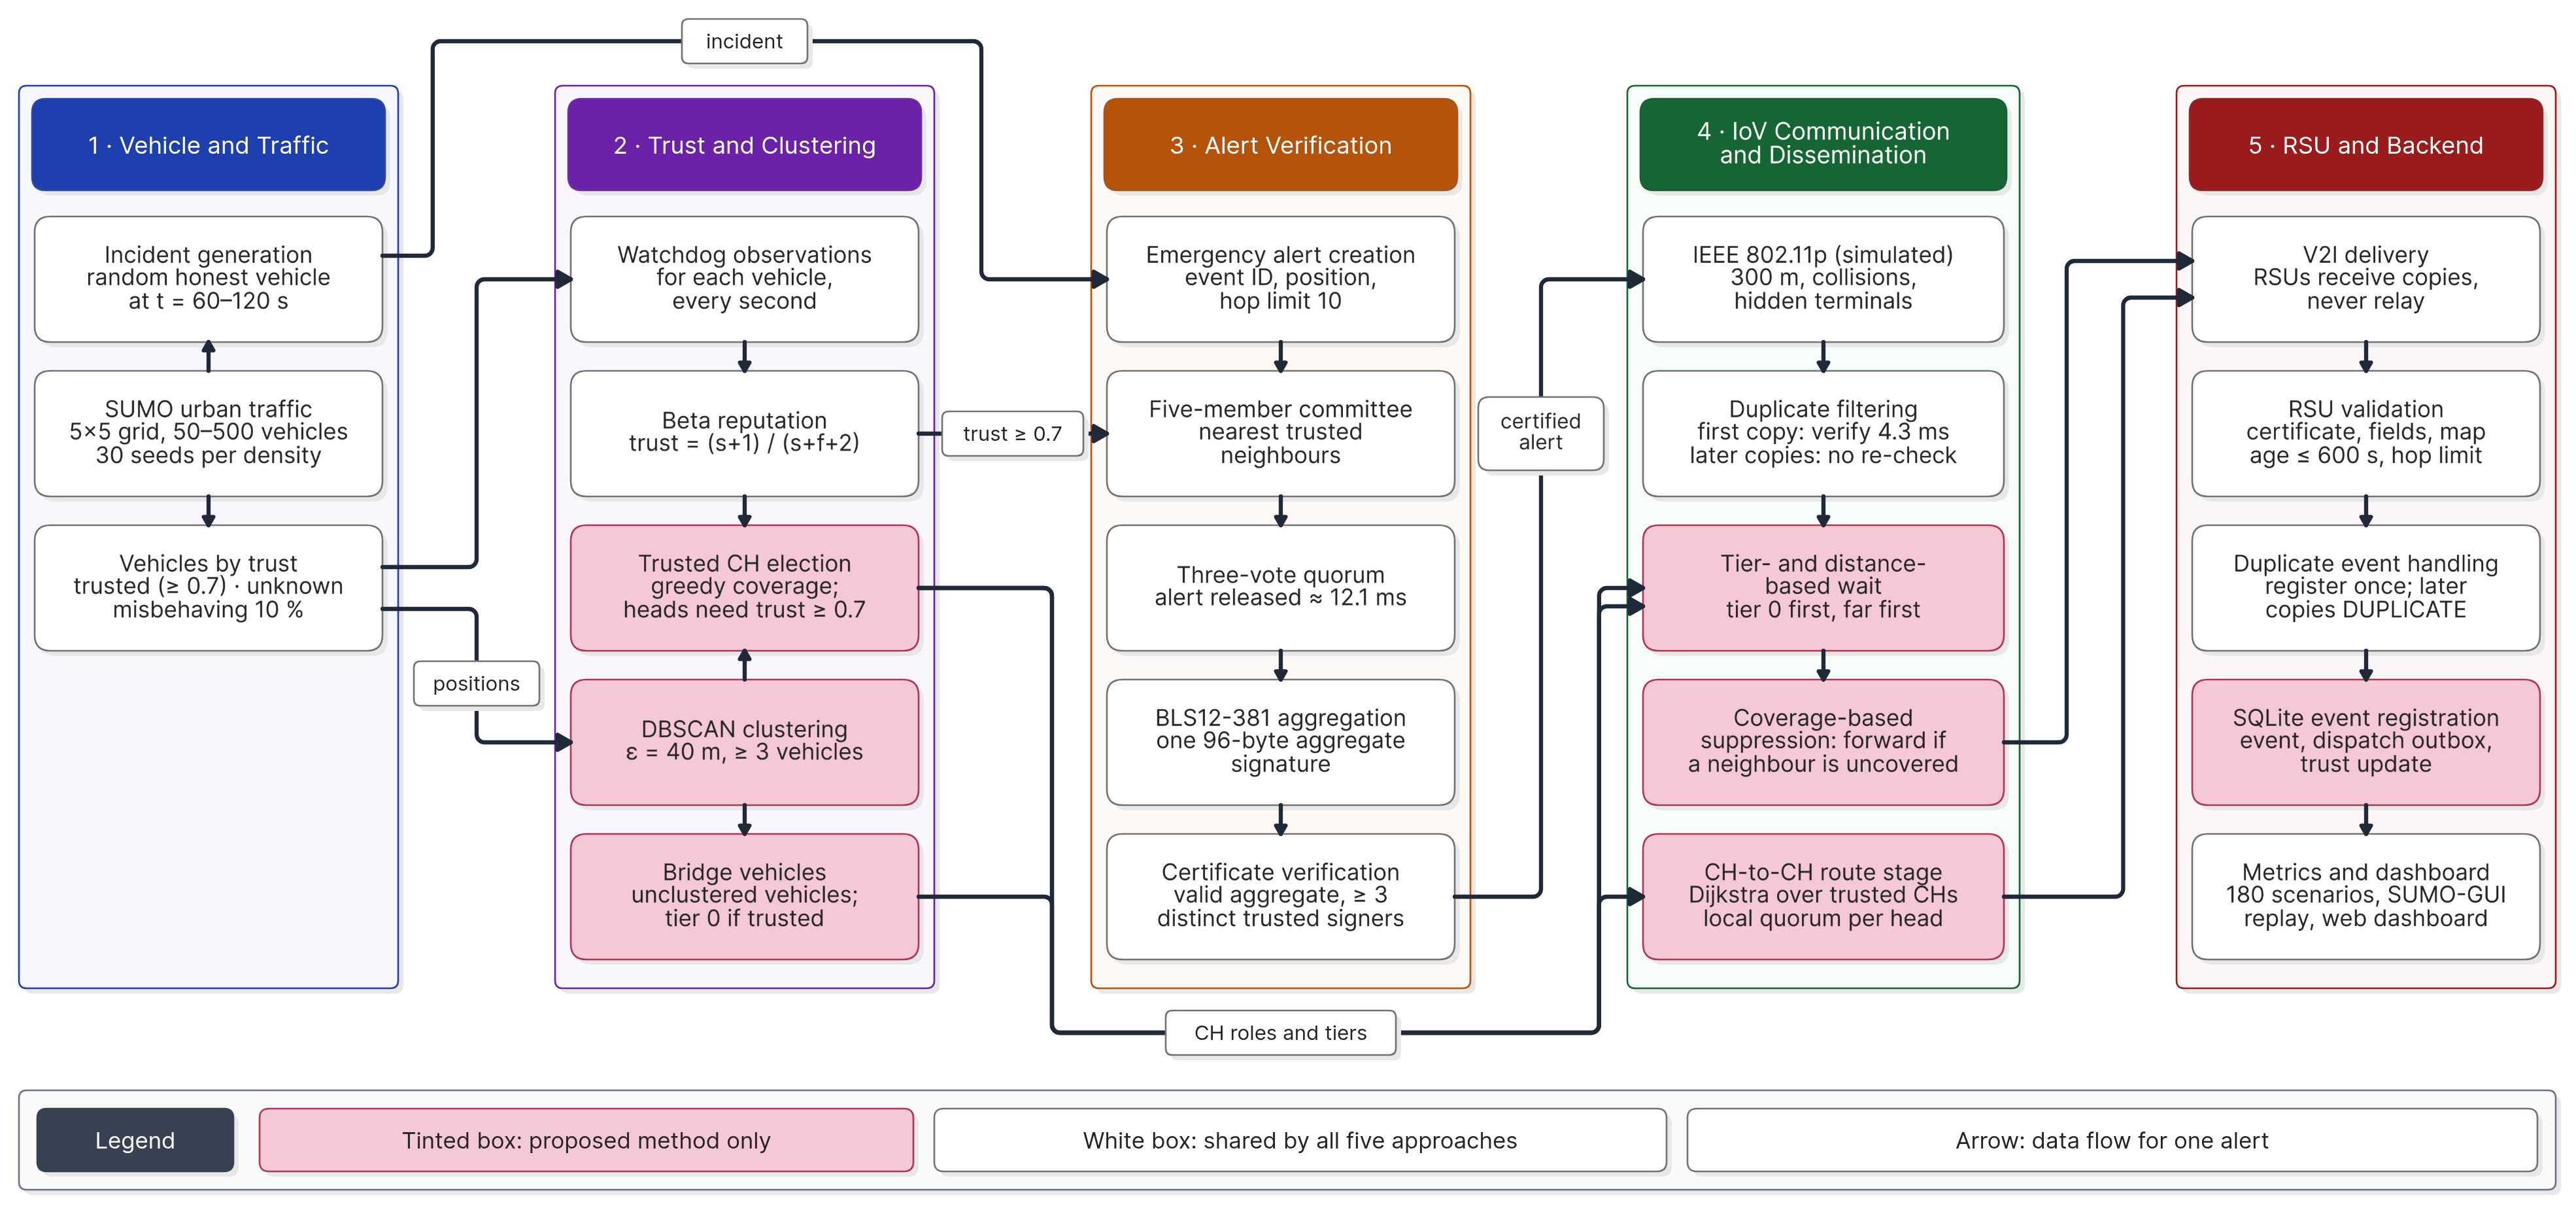
\includegraphics[width=\linewidth,height=0.84\textheight,keepaspectratio]{system_architecture.png}
\caption{System architecture of the implemented pipeline (Eraser.io; source and module list in
\texttt{architecture/}). Read left to right. Tinted boxes are used only by the proposed method; white boxes are shared
by all five approaches. Arrows run only in the gaps between layers and carry the data named on them: the incident
starts the alert, trust selects the committee, the certified alert enters the channel, CH roles and tiers drive the
wait and the route, and forwarded copies reach the RSUs, which register the event once.}
\label{fig:arch}
\end{figure}
\end{landscape}

\begin{table}[H]
\centering
\footnotesize
\renewcommand{\arraystretch}{1.2}
\begin{adjustbox}{max width=\textwidth}
\begin{tabular}{|>{\raggedright\arraybackslash}p{3.2cm}|>{\raggedright\arraybackslash}p{7.6cm}|>{\raggedright\arraybackslash}p{4.8cm}|}
\hline
\textbf{Producer} & \textbf{Data handed over} & \textbf{Consumer} \\
\hline
SUMO (layer 1) & Per-second positions, speeds and lanes; the incident vehicle and second & Watchdog, DBSCAN, alert creation \\
\hline
Watchdog, Beta trust (2) & One trust value per vehicle & CH election, committee, certificate check \\
\hline
CH election (2) & Role (CH, BRIDGE, MEMBER) and tier (0 or 1) per vehicle & Forwarding wait, CH-to-CH route \\
\hline
Committee, BLS (3) & Certified alert: alert fields, signer IDs, one 96-byte aggregate signature & Radio channel \\
\hline
Radio channel (4) & Decoded copies with sender and time; collisions & Duplicate filter, receivers, RSUs \\
\hline
Receivers (4) & Decision per vehicle: FORWARD, SUPPRESS, DROP, EXPIRED or REJECT & Radio channel (next hop), metrics \\
\hline
RSUs (5) & Copy status: REGISTERED, DUPLICATE or REJECTED with reason & SQLite store, metrics, dashboard \\
\hline
Experiment (5) & One record per run (\texttt{results/urban/raw/}), CSV summaries & Charts, replay, dashboard \\
\hline
\end{tabular}
\end{adjustbox}
\caption{How the modules communicate: what each one produces and who uses it.}
\label{tab:interfaces}
\end{table}

% =====================================================================
\section{Technologies Used}
\begin{table}[htbp]
\centering
\footnotesize
\renewcommand{\arraystretch}{1.2}
\begin{adjustbox}{max width=\textwidth}
\begin{tabular}{|p{3.6cm}|p{2.0cm}|p{9.6cm}|}
\hline
\textbf{Technology} & \textbf{Version} & \textbf{Used for} \\
\hline
Python & 3.11.4 & All project code (about 5{,}200 lines in the main modules) \\
SUMO, TraCI, sumolib \cite{lopez2018sumo} & 1.27.1 & Road network, vehicle traffic, incident snapshot; SUMO-GUI for the live demonstration \\
py\_ecc & 8.0.0 & BLS12-381 signing, aggregation and verification \cite{boneh2004short} \\
scikit-learn & 1.7.2 & DBSCAN clustering \cite{ester1996dbscan} \\
NumPy, SciPy & 2.2.6, 1.17.1 & Neighbour tables, statistics (95\,\% Student-t confidence intervals) \\
Matplotlib, Pillow & 3.10.9, 13.0 & Result charts, screenshot processing \\
SQLite (Python standard library) & -- & Local event store, trust table and dispatch outbox \\
HTML, JavaScript, Python \texttt{http.server} & -- & Web dashboard (\texttt{python run.py web}) \\
pytest & 9.1.1 & Validation suite: 105 tests in \texttt{validation/} \\
Eraser.io, \LaTeX{} & -- & Architecture diagram and these documents \\
\hline
\end{tabular}
\end{adjustbox}
\caption{Software used in the implementation.}
\end{table}

\noindent\textbf{Hardware.} All runs were made on one laptop: AMD Ryzen 7 5800H (8 cores, 16 threads), 15.3 GB RAM,
Windows 11. No GPU is used. The full experiment (\NScenarios{} scenarios, all schemes, ablations and the forged-alert
test) takes about 162 s with \texttt{python run.py experiment} (measured on 14 Nov 2026).

\noindent\textbf{Source code.} The public repository \texttt{\RepoURL} was last pushed on 27 Oct 2026; the work
described in this report after that date is in the project folder and not yet pushed. In the project folder one command
reproduces every result: \texttt{python run.py experiment}.

% =====================================================================
\section{Complete End-to-End Implementation}
\label{sec:impl}
Figure~\ref{fig:workflow} shows the 13 stages of one run in execution order. Each stage below lists what it does, why it
is needed, what it receives and produces, and where its output goes.

\begin{figure}[H]
\centering
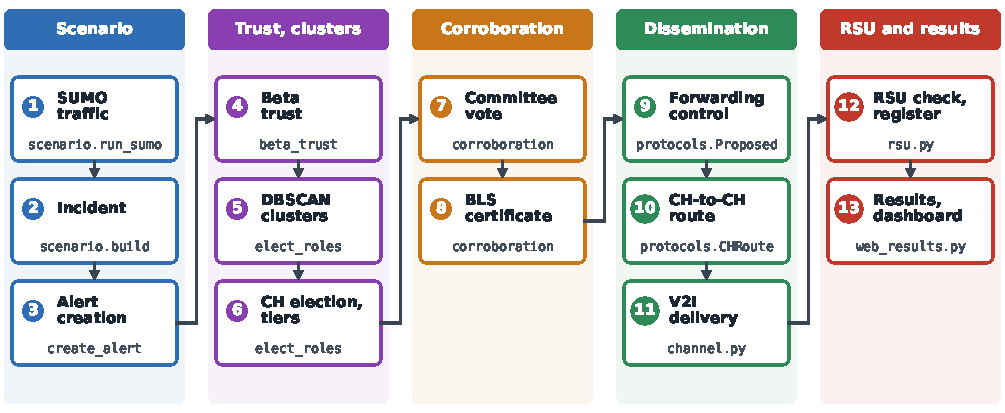
\includegraphics[width=\textwidth]{workflow_pipeline.pdf}
\caption{The 13 stages of one simulated incident in execution order, grouped into five phases (explanatory diagram;
under each stage, the function or module that implements it). Stages 4--6 use the SUMO snapshot at the incident
second; stages 7--12 run in simulated radio time, tens of milliseconds in total.}
\label{fig:workflow}
\end{figure}

\subsection{Stage 1: SUMO traffic}
\stage{Generates vehicle traffic on a straight $5\times5$ urban grid (820 m $\times$ 800 m, 9 signalised junctions, a
three-lane central boulevard). Vehicles enter during the first 30 s and drive random routes of 30 road segments.}
{Positions, speeds and lanes must come from a real traffic model, not from random points.}
{Density $d$ (50 to 500 vehicles) and run index $r$; seed $= 10000 + 100d + r$.}
{Per-second positions, speeds and lanes of every vehicle (SUMO floating car data).}
{Stage 2 (incident) and Stage 4 (trust observations).}

\subsection{Stage 2: Incident generation}
\stage{Draws the incident second uniformly between 60 and 120 s and picks a random honest vehicle on the road at that
second as the crashed vehicle. The same seed always gives the same incident; different seeds give different ones.}
{One reproducible accident per scenario, at a place where traffic is already mixed.}
{The seeded random generator and the traffic of Stage 1.}
{The source vehicle, its position and lane, and a snapshot of all vehicles at that second.}
{Stage 3. All dissemination runs on this snapshot: the slowest one lasts 64 ms, during which a vehicle moves at most
1.25 m.}

\subsection{Stage 3: Alert creation}
\stage{The crashed vehicle builds one alert, similar to an ETSI DENM \cite{etsi302637_3}: event ID, type ACCIDENT, source,
sequence number, position, incident time, creation time and hop limit 10 \cite{etsi302636_4_1}.}
{Receivers and the RSU need a unique event ID to detect duplicates and fixed fields to check.}
{Source vehicle, position, time.}
{A 300-byte alert, e.g. \texttt{EVT-30002-v164-1} in scenario d200\_r02.}
{Stage 7 (the committee must corroborate it before release).}

\subsection{Stage 4: Trust evaluation}
\stage{Every second, each vehicle that has a neighbour is observed once (watchdog \cite{marti2000watchdog}). A
misbehaving vehicle fails the observation; an honest one is misjudged with probability 0.10. Trust is the Beta reputation
$(s+1)/(s+f+2)$ \cite{josang2002beta}.}
{Only vehicles with a good record should lead clusters, vote on alerts or count as endorsers.}
{Per-second neighbour tables and each vehicle's behaviour.}
{A trust value per vehicle; trusted means 0.7 or more.}
{Stage 6 (CH election) and Stage 7 (committee).}

\subsection{Stage 5: Clustering}
\stage{Runs DBSCAN on the vehicle positions with a 40 m radius and at least 3 vehicles per cluster
\cite{ester1996dbscan,chen2024dnov}. A vehicle in no cluster is a \emph{bridge}.}
{Groups give structure: a few well-placed vehicles can cover a whole group.}
{Vehicle positions at the incident second.}
{A cluster label per vehicle, or $-1$ for bridge vehicles.}
{Stage 6.}

\subsection{Stage 6: Cluster-head election}
\stage{In each cluster, repeatedly picks the trusted member whose 300 m radio range covers the most still-uncovered
members (greedy set cover); ties go to the vehicle with the lowest speed difference to its neighbours. A cluster without
trusted members gets no CH.}
{CHs and trusted bridges forward first (tier 0), so the alert takes a short, reliable path through each cluster.}
{Clusters, trust, speeds and the neighbour table.}
{A role per vehicle (CH, BRIDGE, MEMBER) and a tier (0 or 1). In d200\_r02: 20 clusters, 20 CHs, 37 isolated vehicles.}
{Stage 9 (tiers) and Stage 10 (route over trusted CHs).}

\subsection{Stage 7: Committee voting}
\stage{The source sends a signed proposal. The five nearest in-range neighbours with trust $\geq 0.7$ form the committee.
A member that observed the event checks the proposal and returns a 132-byte vote in rank order (0.5 ms apart). The source
counts each distinct voter once and releases the alert at three votes.}
{A single vehicle must not be able to start an alert on its own.}
{The alert, the neighbour table and trust.}
{At least three distinct signatures; the certified alert is released about \NQuorumMs{} ms after the incident.}
{Stage 8.}

\subsection{Stage 8: Authentication (BLS certificate)}
\stage{Merges the source's and the voters' BLS12-381 signatures over a digest of all alert fields into one 96-byte
aggregate. A receiver accepts the alert only if the first signer is the source, the signers are distinct, the aggregate
verifies, and at least three endorsers are trusted (an unknown signer counts as 0).}
{Changing any field breaks the signature, and colluders with a poor record cannot form a valid certificate.}
{Votes and the alert.}
{The certified alert (alert, signer IDs, aggregate signature). Simulated cost: 1.4 ms to sign, 4.3 ms to verify
(configured processing times).}
{Stage 9 via the radio channel.}

\subsection{Stage 9: Forwarding control (duplicate filter and controlled broadcast)}
\stage{The radio model (\texttt{channel.py}) is slot-level IEEE 802.11p: 6 Mbit/s, 13\,$\mu$s slots, AC\_VO access,
broadcast without acknowledgement, 300 m range, collisions, hidden terminals and half duplex. When a vehicle decodes the
first copy of an event, it verifies the certificate (4.3 ms) and accepts or rejects it. A later copy of the same event is
never verified again: it only adds its sender to the set of heard senders. An accepted vehicle sets a timer
(equation~\ref{eq:timer}) and, when it fires, forwards only if one of its neighbours is not covered by any heard sender
(equation~\ref{eq:cover}).}
{This is where the broadcast storm is controlled: far vehicles and tier-0 vehicles go first, and covered areas stay
silent.}
{Received copies, tiers, the neighbour table.}
{A decision per vehicle: FORWARD, SUPPRESS, DROP (misbehaving), EXPIRED (hop limit) or REJECT, each with its reason.}
{Stage 11 (an RSU in range receives the copy) and further receivers.}

\begin{equation}
T = t_{acc} + \bigl(\mathrm{tier}\cdot N_s + S(d)\bigr)\,\tau + U[0,\mathrm{RAD}), \qquad
S(d) = \min\!\Bigl(N_s-1,\ \max\bigl(0,\ N_s - \lceil N_s \min(d,R)/R \rceil \bigr)\Bigr)
\label{eq:timer}
\end{equation}
with $N_s = 5$ slots, $\tau = 5$ ms, RAD $= 5$ ms and $R = 300$ m. Farther receivers get earlier slots.
\begin{equation}
\text{forward} \iff N(v) \setminus \bigcup_{h \in H(v)} \bigl(N(h) \cup \{h\}\bigr) \neq \emptyset
\label{eq:cover}
\end{equation}
where $N(v)$ is the set of neighbours of $v$ (vehicles and RSUs) and $H(v)$ the senders $v$ has heard.

\subsection{Stage 10: CH-to-CH routing}
\stage{Computes the shortest path by distance (Dijkstra) from the source to the nearest RSU over CHs with trust
$\geq 0.7$. Each head on the route collects a local quorum (itself plus two cluster votes) before forwarding; vehicles off
the route stay silent.}
{It gives the RSU a short, corroborated delivery path with very few frames.}
{Roles, trust, positions and the certified alert.}
{A route such as \texttt{v164 $\rightarrow$ v32 $\rightarrow$ RSU-2} (d200\_r02) and the frames sent along it.}
{Stage 11. There is no fallback: a missing route or a failed local quorum means no delivery on this path (reported).}

\subsection{Stage 11: V2I delivery}
\stage{Treats RSUs as ordinary neighbours in the coverage test of Stage 9, so a vehicle with an uncovered RSU nearby
forwards; the CH route ends at an RSU. RSUs only receive, they never relay.}
{The alert reaches the infrastructure without a separate routing protocol in the broadcast.}
{Forwarded copies near RSU-1 (160, 590) m and RSU-2 (610, 170) m, placed at intersections \cite{trullols2010rsu}.}
{RSU receptions: RSU, sender, arrival time, hop count.}
{Stage 12.}

\subsection{Stage 12: RSU verification and registration}
\stage{Takes the copies in arrival order. For each, it verifies the certificate (4.3 ms) and checks that all fields are
present, the type is known, the position lies inside the map, the alert was not created after reception, it is not older
than 600 s on the RSU's own clock \cite{etsi302637_3}, and the hop count is within the limit. The first valid copy is
REGISTERED; later copies of the same event at any RSU are DUPLICATE; failures are REJECTED with the reason.}
{One accident must create exactly one event for the traffic centre, and implausible or uncorroborated alerts must stop
here.}
{RSU receptions and the certificate.}
{The registered event (receiving RSU, delay, hops) and the status of every copy.}
{Stage 13. The event delivered by the CH-to-CH route stage is written to a local SQLite store and dispatch outbox, and the
vehicles that forwarded it receive a small trust increase, $T' = (20T + 1)/21$.}

\subsection{Stage 13: Results and dashboard}
\stage{Computes the metrics of every scheme from the channel log and protocol state, writes one record per run
(\texttt{results/urban/raw/}), aggregates mean and 95\,\% confidence intervals (\texttt{processed/summary.csv}) and paired
differences, and draws the charts. The same records drive the SUMO-GUI replay and the web dashboard.}
{Results must be reproducible and traceable; nothing is typed in by hand.}
{All run records.}
{CSV summaries, \texttt{RESULTS.md}, figures, the replay and the dashboard (Sections~\ref{sec:sumo}--\ref{sec:results}).}
{The panel and the reader.}

% =====================================================================
\section{Algorithm Implementation and Comparison}
\label{sec:algos}
All five approaches are implemented in \texttt{protocols.py} as subclasses of one \texttt{Protocol} class. They share the
same corroboration (committee, BLS certificate, acceptance rule), the same radio model, the same duplicate bookkeeping
(a vehicle processes only its first copy) and the same RSU. They differ only in \emph{when} and \emph{whether} a vehicle
rebroadcasts.

\begin{enumerate}[noitemsep, topsep=2pt]
  \item \textbf{Blind flooding.} Every vehicle that accepts the alert rebroadcasts it once, immediately after verification.
  \item \textbf{Flooding with random delay.} As flooding, but each rebroadcast waits a random delay $U[0, 5\text{ ms})$
        \cite{ni1999broadcast}, which spreads transmissions over time.
  \item \textbf{Slotted 1-persistence} \cite{wisitpongphan2007}. A receiver waits $S(d)\cdot\tau$ (farther receivers wait
        less) and cancels if it hears a duplicate before its slot.
  \item \textbf{Slotted 1-persistence with random delay.} As above, plus the same random delay inside the slot. This is
        the strongest baseline: it isolates what tiers and the coverage test add beyond jitter.
  \item \textbf{Proposed.} Trust-aware tiers, distance slots, random delay and the coverage test
        (equations~\ref{eq:timer}--\ref{eq:cover}), plus the CH-to-CH route stage.
\end{enumerate}

\begin{table}[htbp]
\centering
\footnotesize
\renewcommand{\arraystretch}{1.2}
\begin{adjustbox}{max width=\textwidth}
\begin{tabular}{|>{\raggedright\arraybackslash}p{2.6cm}|>{\raggedright\arraybackslash}p{3.1cm}|>{\raggedright\arraybackslash}p{2.5cm}|>{\raggedright\arraybackslash}p{3.0cm}|>{\raggedright\arraybackslash}p{2.0cm}|>{\raggedright\arraybackslash}p{2.2cm}|}
\hline
\textbf{Approach} & \textbf{Forwarding rule} & \textbf{Delay before relaying} & \textbf{Duplicate handling} & \textbf{Verification} & \textbf{Routing} \\
\hline
Blind flooding & Every accepting vehicle relays once & None & Counted only; never suppress & Shared & None \\
\hline
Flooding + random delay & Every accepting vehicle relays once & $U[0, 5\text{ ms})$ & Counted only; never suppress & Shared & None \\
\hline
Slotted 1-persistence & Relay at slot $S(d)$ unless a duplicate arrives first & Distance slot & Any duplicate before the slot cancels & Shared & None \\
\hline
Slotted 1-p + random delay & As slotted 1-p & Distance slot + random delay & As slotted 1-p & Shared & None \\
\hline
Proposed & Relay only if a neighbour is uncovered & Tier + distance slot + random delay & Duplicates mark neighbours as covered & Shared & CH-to-CH route stage (local quorum per head) \\
\hline
\end{tabular}
\end{adjustbox}
\caption{How the five implemented approaches forward an alert. ``Shared'' = the same committee voting, BLS certificate
and acceptance rule for every approach.}
\label{tab:mech}
\end{table}

\noindent\textbf{Shared and specific mechanisms.} Committee voting, BLS aggregation, the receiver's certificate check,
the duplicate bookkeeping, the radio model, the hop limit and the RSU validation are \emph{shared} by all five approaches,
so security costs the same in every column of the results. \emph{Specific} to the proposed method are the trust-aware
CH election and tiers, the coverage test and the CH-to-CH route stage with its per-head local quorum. To measure each
specific part, the experiment also runs the proposed method with one component removed (ablations): without random delay,
without distance slots, without coverage test, without clustering, without cluster-based forwarding, without reputation
gate, and without voting + BLS. Section~\ref{sec:results} reports, metric by metric, where the proposed method is
better than each baseline, where it is similar and where it is worse.

% =====================================================================
\section{SUMO Traffic and Accident Simulation}
\label{sec:sumo}
Table~\ref{tab:scenario} lists the scenario parameters. The figures in this section are captures of the live SUMO-GUI
window from one complete run of the full walkthrough (\texttt{python run.py demo}), scenario d200\_r02 (200 vehicles,
seed 30002, vehicle v164 crashes at (684, 588) m at $t = 114$ s). This is the fixed showcase scenario of the demo; the
experiment and the comparison pairs use a different seeded incident in every scenario. The radio events last tens of
milliseconds, so the replay pauses the SUMO clock and shows them in slow motion. The run's record fingerprint
(397f81ab\ldots) matches the experiment's record of this seed. Figure~\ref{fig:sumo_window} shows the whole window
once, with its legend and status lines; Figures~\ref{fig:sumo_incident}--\ref{fig:sumo_final} show the map area of the
same window, enlarged, with the status lines repeated in full width where they carry the result. Every image is a crop
of a capture; nothing in it is drawn or edited.

\begin{table}[htbp]
\centering
\footnotesize
\renewcommand{\arraystretch}{1.2}
\begin{adjustbox}{max width=\textwidth}
\begin{tabular}{|p{4.2cm}|p{11.4cm}|}
\hline
Road network & Straight $5\times5$ urban grid, 820 m $\times$ 800 m, 9 signalised junctions, 3-lane central boulevard (\texttt{network/urban.net.xml}) \\
\hline
Traffic densities & 50, 100, 200, 250, 300 and 500 vehicles; 30 seeds each (\NScenarios{} scenarios) \\
\hline
Seeds & $\text{seed} = 10000 + 100 \cdot \text{density} + \text{run}$; every run is reproducible \\
\hline
Incident & One honest vehicle at a random second in [60, 120] s \\
\hline
Misbehaving vehicles & 10\,\% of vehicles; receive but never relay (persistent by default; on-off in a sensitivity sweep) \\
\hline
RSUs & 2, at junctions B3 (160, 590) m and D1 (610, 170) m; the far corners are deliberately outside direct RSU range \\
\hline
Radio & IEEE 802.11p model, 300 m range (150 m and 450 m in a sensitivity sweep), no fading \\
\hline
\end{tabular}
\end{adjustbox}
\caption{Scenario parameters (\texttt{config.py}).}
\label{tab:scenario}
\end{table}

\begin{figure}[H]
\centering
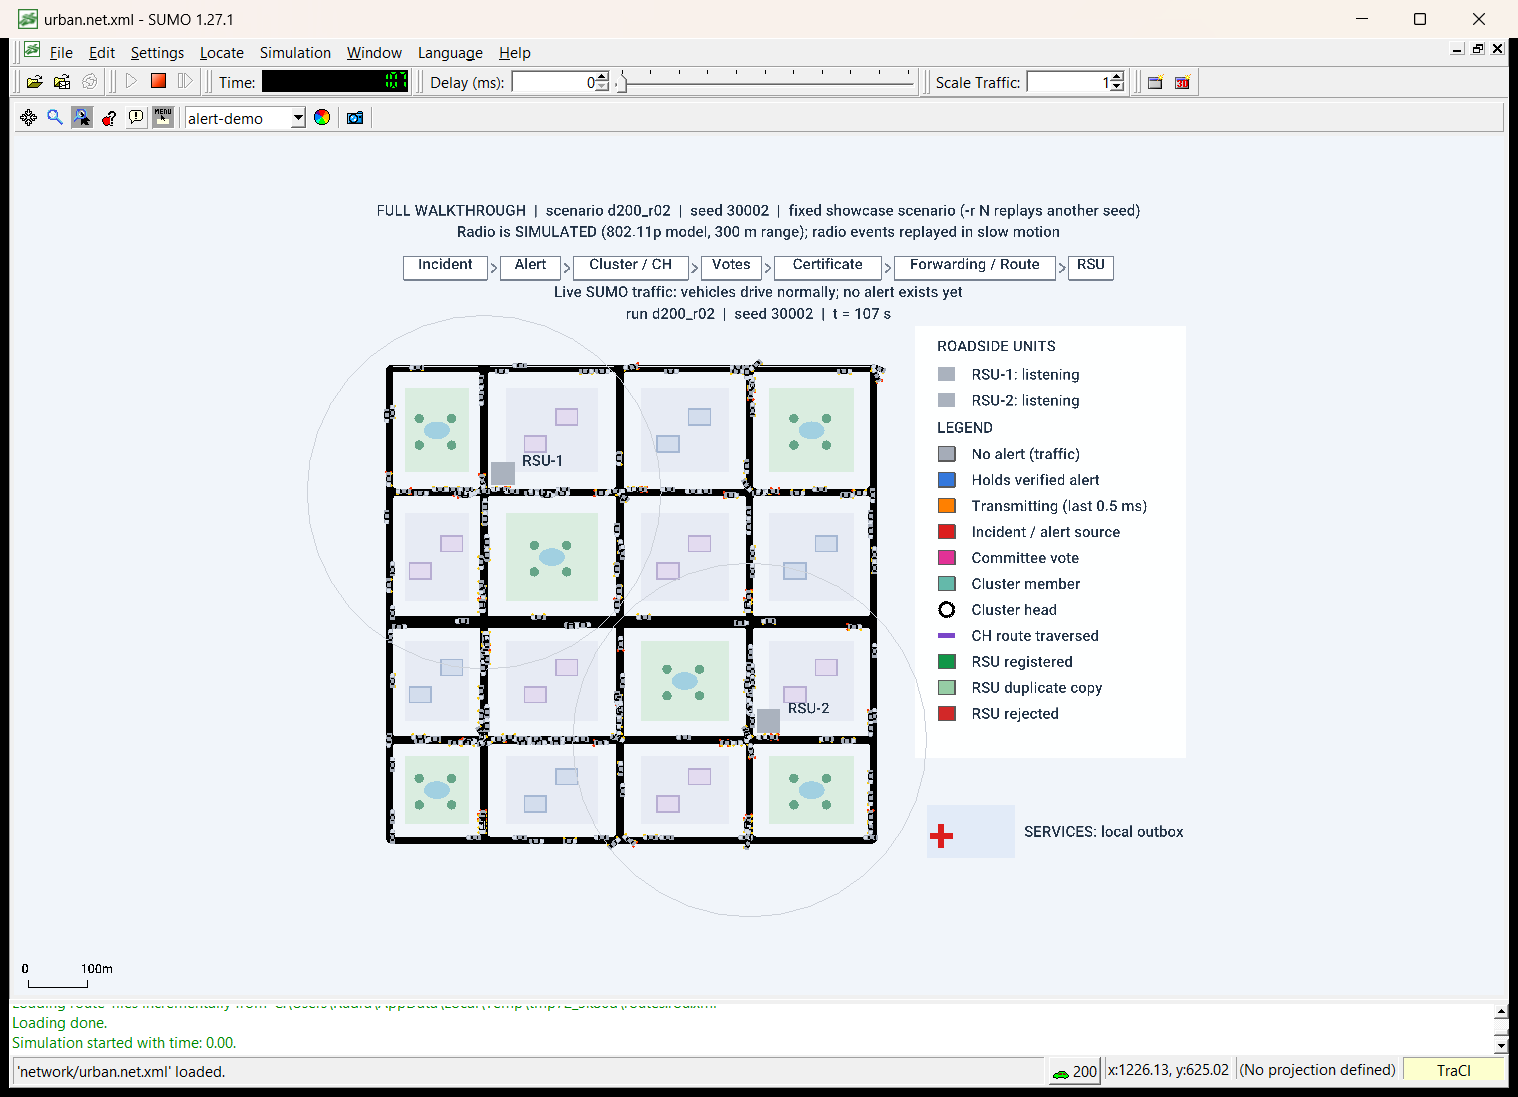
\includegraphics[width=0.96\textwidth]{shot_window_traffic.png}
\caption{SUMO-GUI 1.27.1 running scenario d200\_r02, full window, at $t = 107$ s before the incident.
\emph{Observe:} the label at the top names the run; the stage bar (Incident $\rightarrow$ \ldots{} $\rightarrow$ RSU)
highlights the current step; the two status lines give the live counts; the legend on the right is used by every later
capture (grey: no alert, blue: holds the verified alert, orange ring: transmitting, red: incident or alert source,
magenta: committee vote, black ring: cluster head, purple line: CH route, green: RSU registered, light green: RSU
duplicate copy).}
\label{fig:sumo_window}
\end{figure}

\begin{figure}[H]
\centering
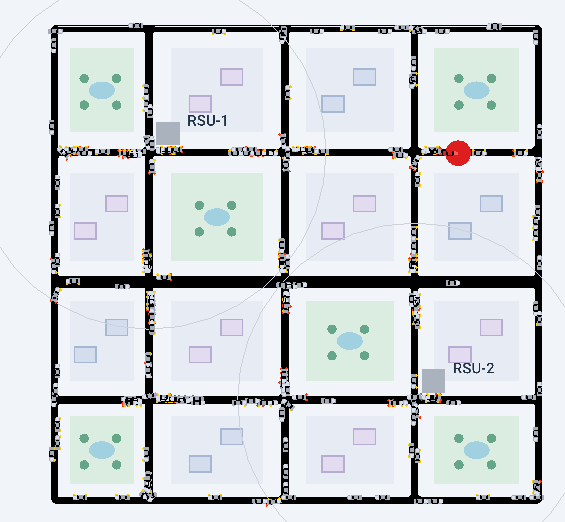
\includegraphics[width=0.49\textwidth]{view_map_walk_02_incident.png}\hfill
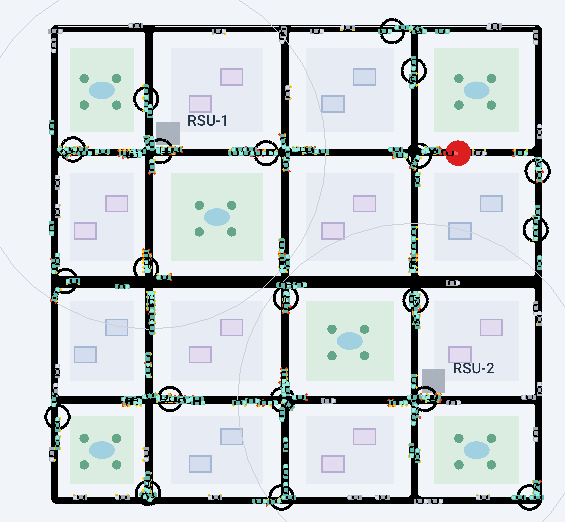
\includegraphics[width=0.49\textwidth]{view_map_walk_04_clusters.png}
\caption{Left: incident generation. \emph{Observe:} the red marker where v164 stops at (684, 588) m at $t = 114$ s;
both RSUs are grey (listening). Right: clustering and CH election on the same snapshot. \emph{Observe:} the black rings,
the 20 cluster heads elected among vehicles with trust $\geq 0.7$, one per DBSCAN cluster (40 m); the 37 vehicles in no
cluster are bridges.}
\label{fig:sumo_incident}
\end{figure}

\begin{figure}[H]
\centering
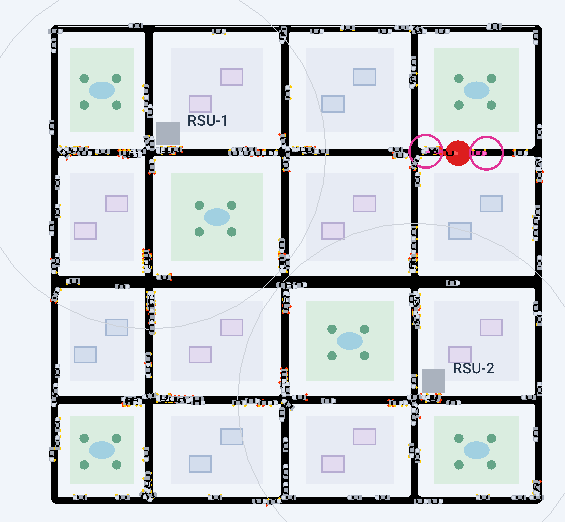
\includegraphics[width=0.49\textwidth]{view_map_walk_05_votes.png}\hfill
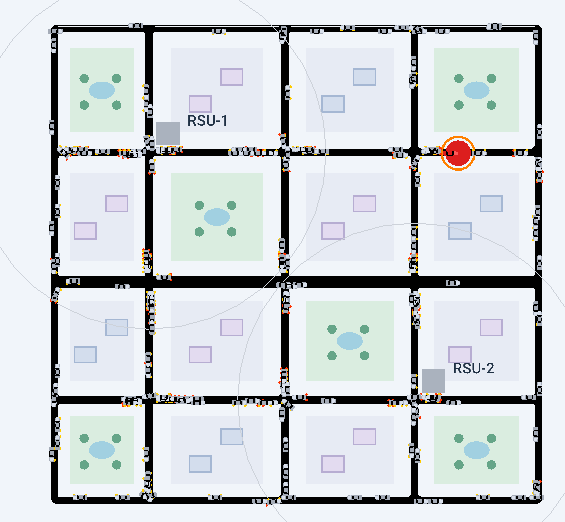
\includegraphics[width=0.49\textwidth]{view_map_walk_06_certificate.png}
\caption{Committee voting and authentication (proposed method). Left: \emph{observe} the magenta rings next to the
source, 2 of the 5 committee members voting (+7.0 ms radio time; 3 votes are needed). Right: \emph{observe} the orange
ring at the source, which transmits the certified alert: 4 BLS signatures merged into one 96-byte aggregate
(+12.5 ms). Receivers verify it before accepting.}
\label{fig:sumo_votes}
\end{figure}

\begin{figure}[H]
\centering
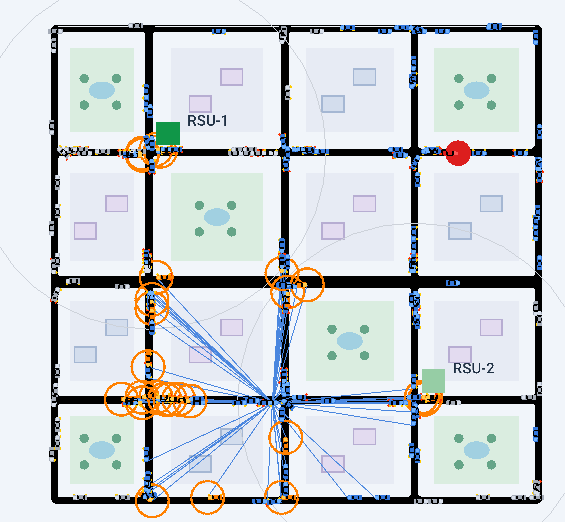
\includegraphics[width=0.49\textwidth]{view_map_walk_07_flooding.png}\hfill
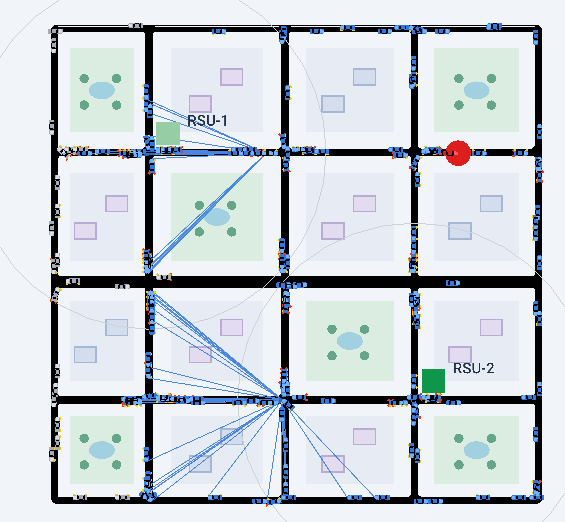
\includegraphics[width=0.49\textwidth]{view_map_walk_09_duplicates.png}\par\smallskip
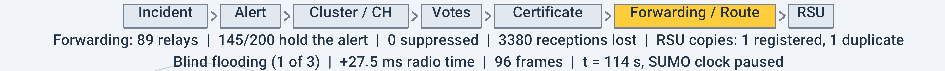
\includegraphics[width=\textwidth]{view_status_walk_07_flooding.png}\par
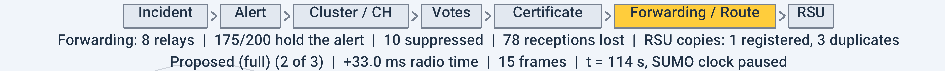
\includegraphics[width=\textwidth]{view_status_walk_09_duplicates.png}
\caption{Same incident, two forwarding rules (one run, an illustration rather than a statistical result). Left and
first status line: blind flooding at +27.5 ms, 89 relays, 145/200 vehicles hold the alert, 3380 receptions lost.
Right and second status line: the proposed method at +33.0 ms, 8 relays, 175/200 hold the alert, 10 vehicles
suppressed, 78 receptions lost. \emph{Observe:} the many orange transmission rings under flooding and the few under the
proposed method, while blue (alert received) spreads over the grid in both.}
\label{fig:sumo_forward}
\end{figure}

\begin{figure}[H]
\centering
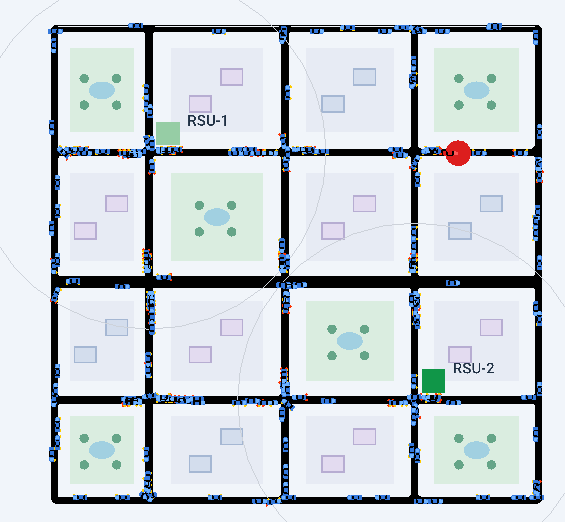
\includegraphics[width=0.49\textwidth]{view_map_walk_10_rsu.png}\hfill
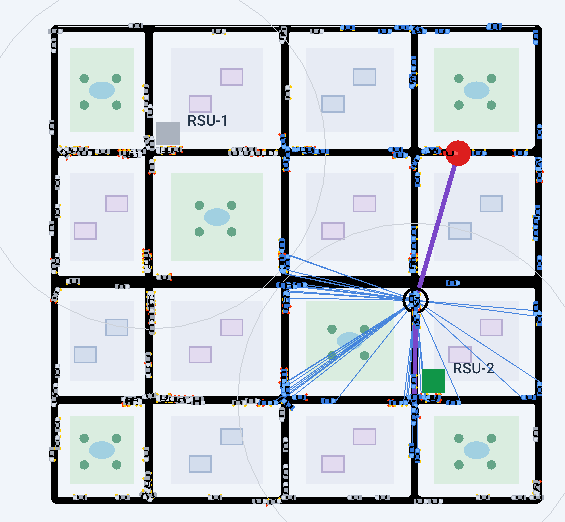
\includegraphics[width=0.49\textwidth]{view_map_walk_11_route.png}
\caption{Left: RSU processing for the proposed broadcast. \emph{Observe:} RSU-2 green, it decoded the alert at
+18.2 ms, verified it and registered it at +22.5 ms; RSU-1 light green, its copies were counted as duplicates
(12 duplicate copies in total). Right: the CH-to-CH route stage. \emph{Observe:} the purple line
v164 $\rightarrow$ v32 $\rightarrow$ RSU-2 through one cluster head; RSU-2 registered the routed copy at +40.6 ms.}
\label{fig:sumo_rsu}
\end{figure}

\begin{figure}[H]
\centering
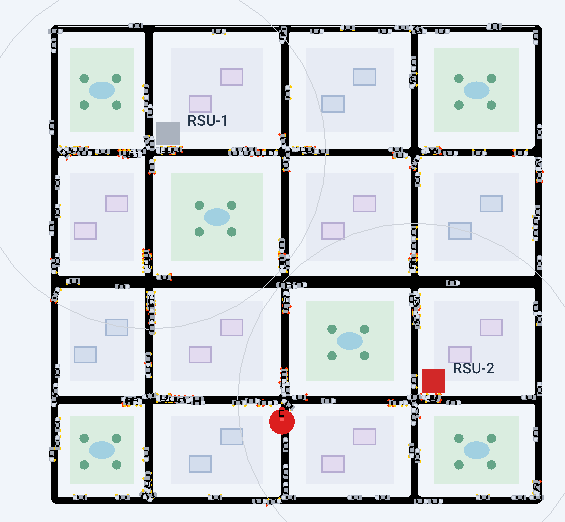
\includegraphics[width=0.49\textwidth]{view_map_walk_12_forged.png}\hfill
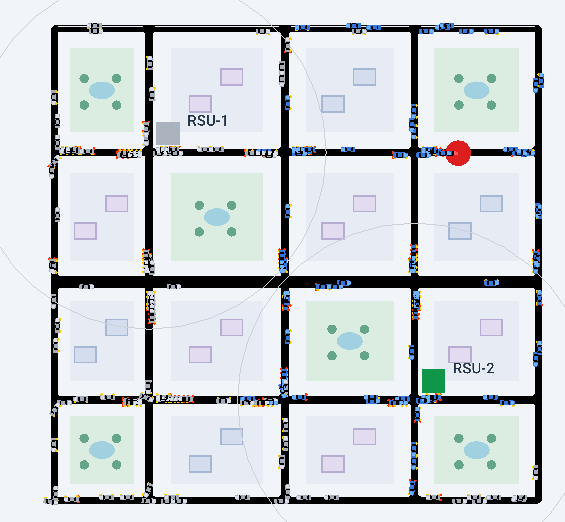
\includegraphics[width=0.49\textwidth]{view_map_walk_13_final.png}\par\smallskip

\includegraphics[width=\textwidth]{view_status_walk_12_forged.png}\par

\includegraphics[width=\textwidth]{view_status_walk_13_final.png}
\caption{Left and first status line: forged-alert test on the same traffic with full protection. \emph{Observe:}
RSU-2 red (rejected) and no blue vehicles: the colluders' certificate has 0 reputable endorsers (3 needed), so the RSU
rejects every copy and no honest vehicle accepts the alert. Right and second status line: final screen. \emph{Observe:}
RSU-2 green, the CH-route delivery registered and the dispatch queued in the local outbox; the SUMO clock runs again.}
\label{fig:sumo_final}
\end{figure}

% =====================================================================
\section{Dashboard and Working Demonstration}
\label{sec:demo}
The demonstration has two parts. \textbf{(1) SUMO-GUI replay} (\texttt{python run.py demo}) shows the full walkthrough
above. \textbf{(2) Comparison pairs} on the web dashboard (\texttt{python run.py web}, then open
\url{http://127.0.0.1:8765/}).
A pair is one incident scenario replayed twice in SUMO-GUI: once with one baseline only and once with the proposed method
only (its CH-to-CH route stage and the forged-alert test included). Only one run can be active at a time. Each run
re-simulates the same seed into its own folder, and the comparison is shown only when both runs' records have the same
fingerprint, which proves both runs used identical traffic, incident and parameters. New pairs take scenarios in an
order shuffled by a random seed kept per pairs folder, so different pairs show different incidents.

\begin{figure}[H]
\centering
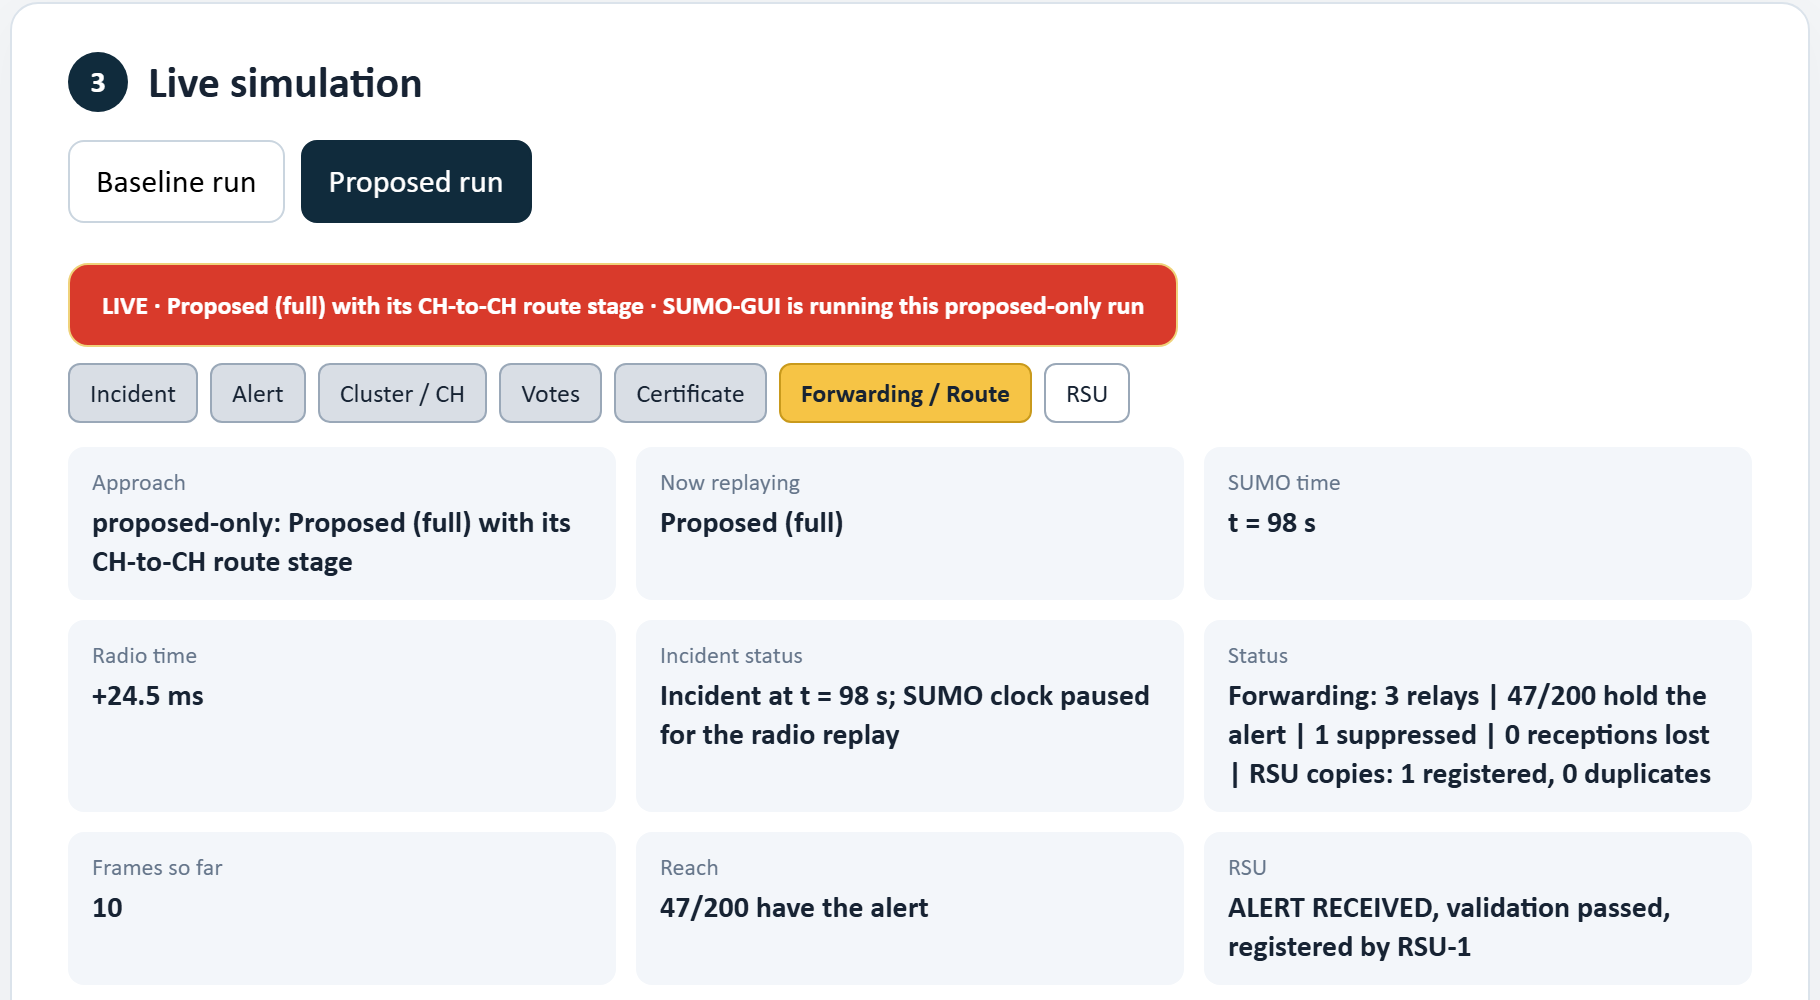
\includegraphics[width=0.74\textwidth]{view_dash_live.png}
\caption{Dashboard section 3 during a live proposed-only run of scenario d200\_r25 (seed 30025), captured on
15 Nov 2026 while SUMO-GUI was running. \emph{Observe:} the red LIVE banner; the highlighted stage
(Forwarding / Route); the radio time (+24.5 ms), reach (47/200 vehicles) and frames so far (10); and the RSU card:
the alert passed validation and RSU-1 registered it. The SUMO-GUI window of the run starts below the cards.}
\label{fig:dash_live}
\end{figure}

\begin{figure}[H]
\centering
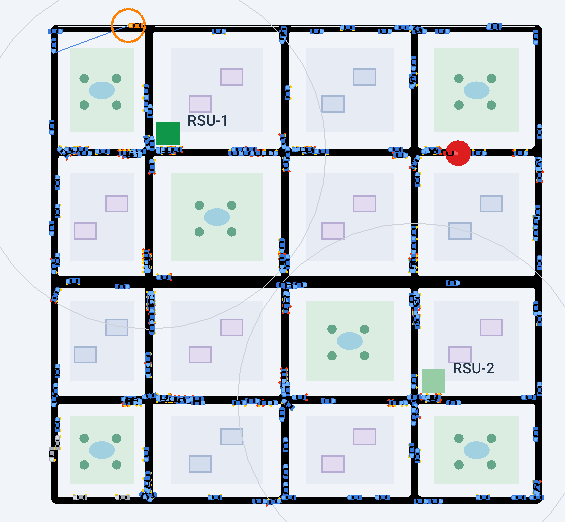
\includegraphics[width=0.45\textwidth]{view_map_P002_baseline_014.png}\hspace{0.03\textwidth}%
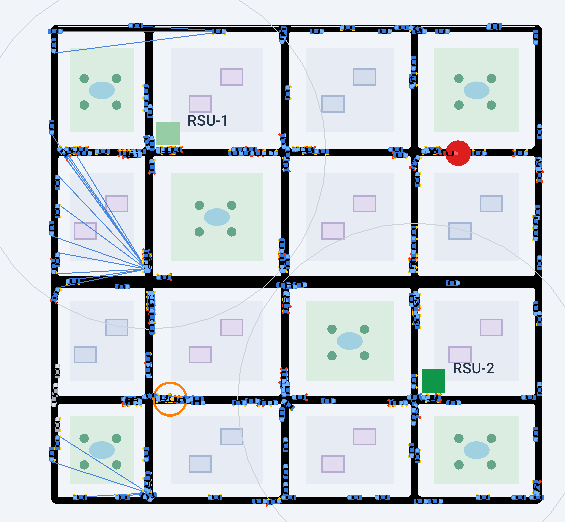
\includegraphics[width=0.45\textwidth]{view_map_P002_proposed_015.png}\par\smallskip
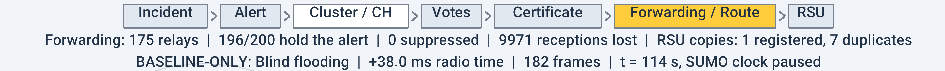
\includegraphics[width=0.93\textwidth]{view_status_P002_baseline_014.png}\par
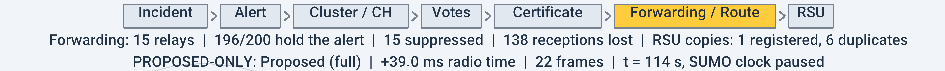
\includegraphics[width=0.93\textwidth]{view_status_P002_proposed_015.png}
\caption{Comparison pair P002 (scenario d200\_r02), captured live in two separate SUMO-GUI runs. Left and first status
line: baseline-only run (blind flooding), +38.0 ms. Right and second: proposed-only run, +39.0 ms. \emph{Observe:} both
maps are almost all blue (196/200 vehicles reached); the status lines show the difference: 175 relays and 9971
receptions lost against 15 relays, 15 suppressed and 138 lost. Both runs replayed one record (fingerprint
397f81ab\ldots).}
\label{fig:pair}
\end{figure}


\begin{figure}[H]
\centering
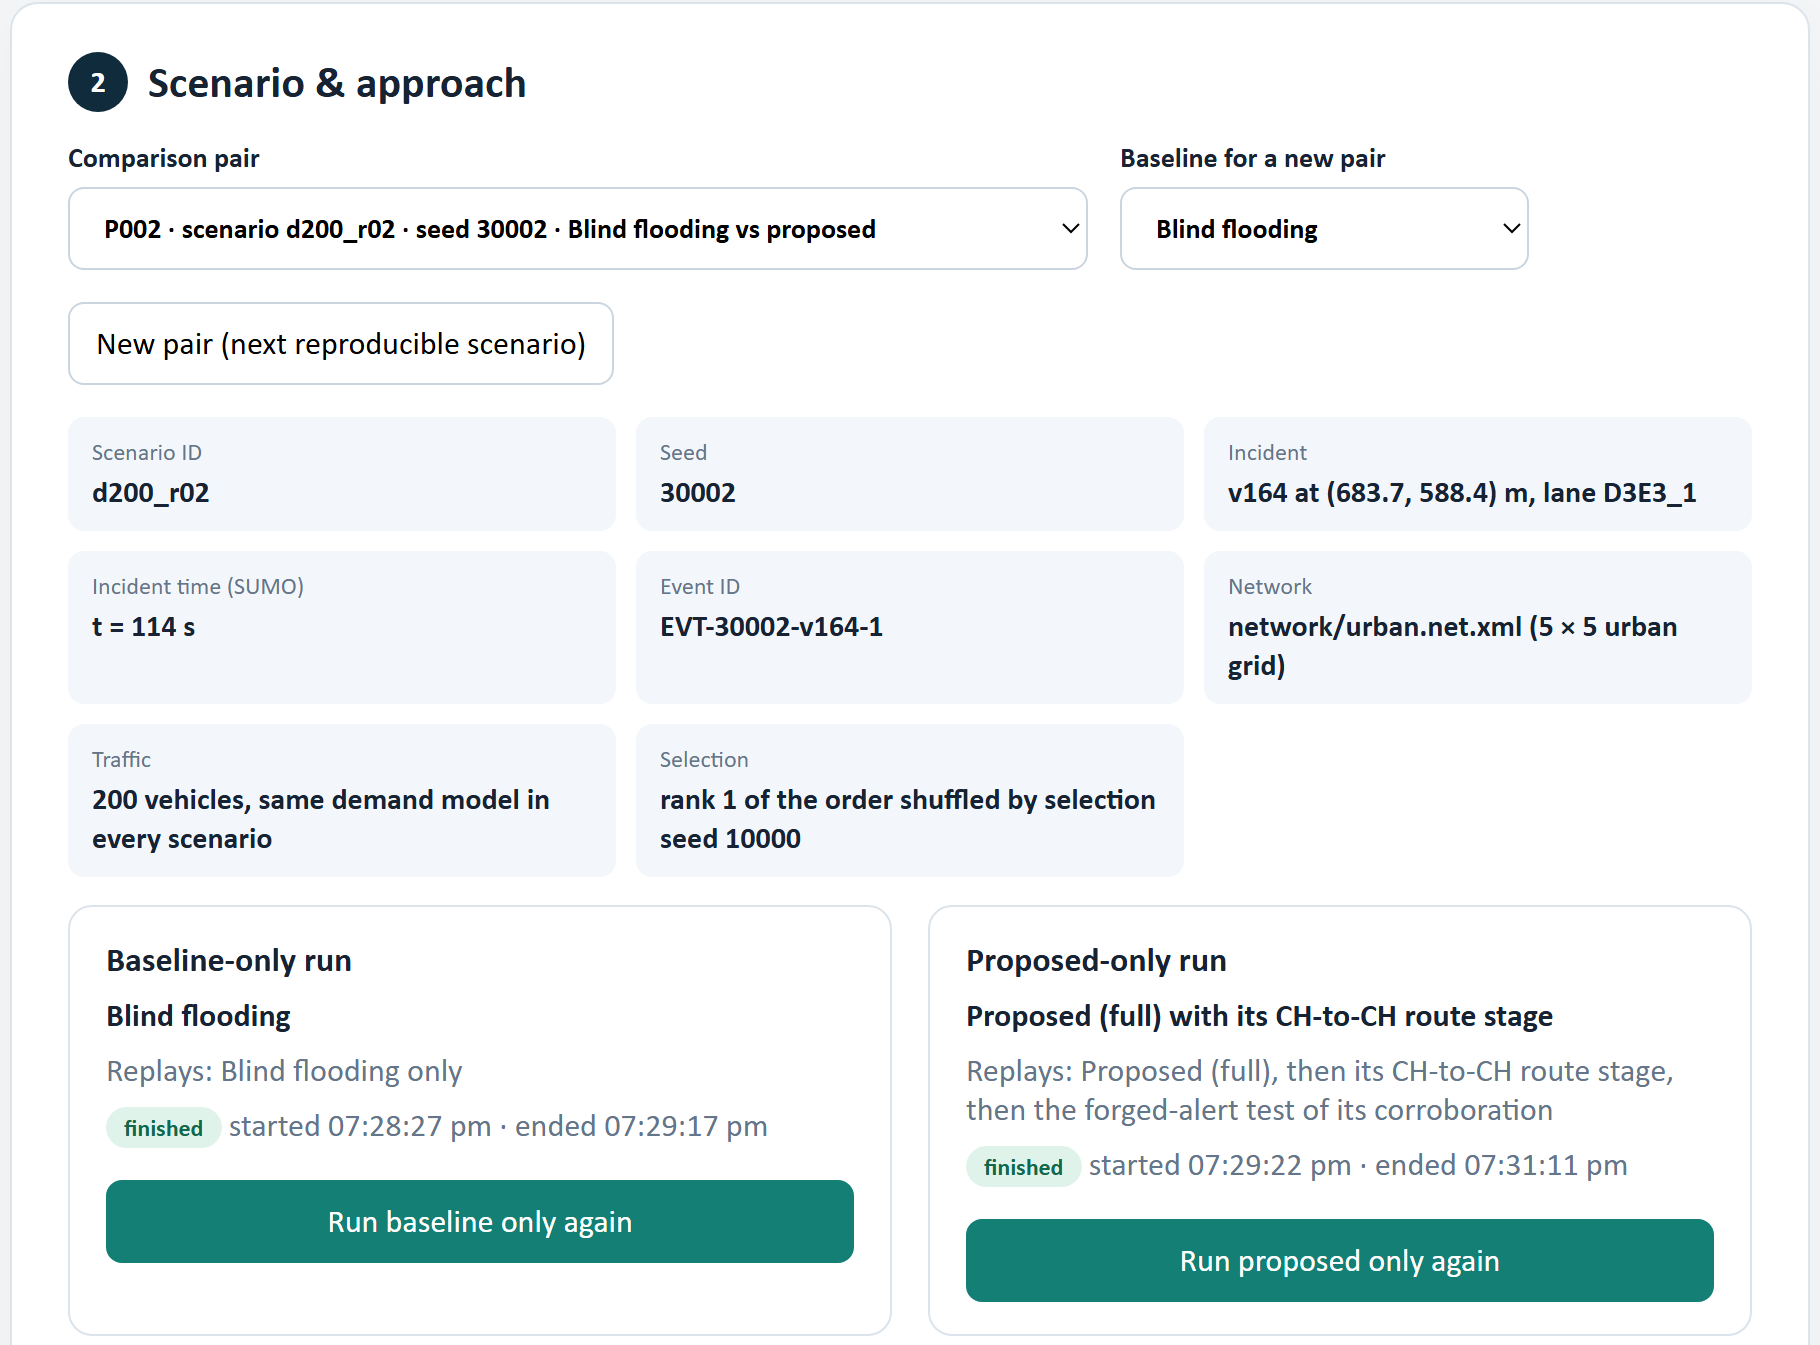
\includegraphics[width=0.8\textwidth]{view_dash_scenario.png}
\caption{Dashboard section 2 for pair P002. \emph{Observe:} the pair selector, the scenario facts (d200\_r02, seed
30002, v164 at $t = 114$ s, event EVT-30002-v164-1) and the two separate runs, baseline-only (blind flooding) and
proposed-only, both marked finished with their start and end times.}
\label{fig:dash_scenario}
\end{figure}

\begin{figure}[H]
\centering
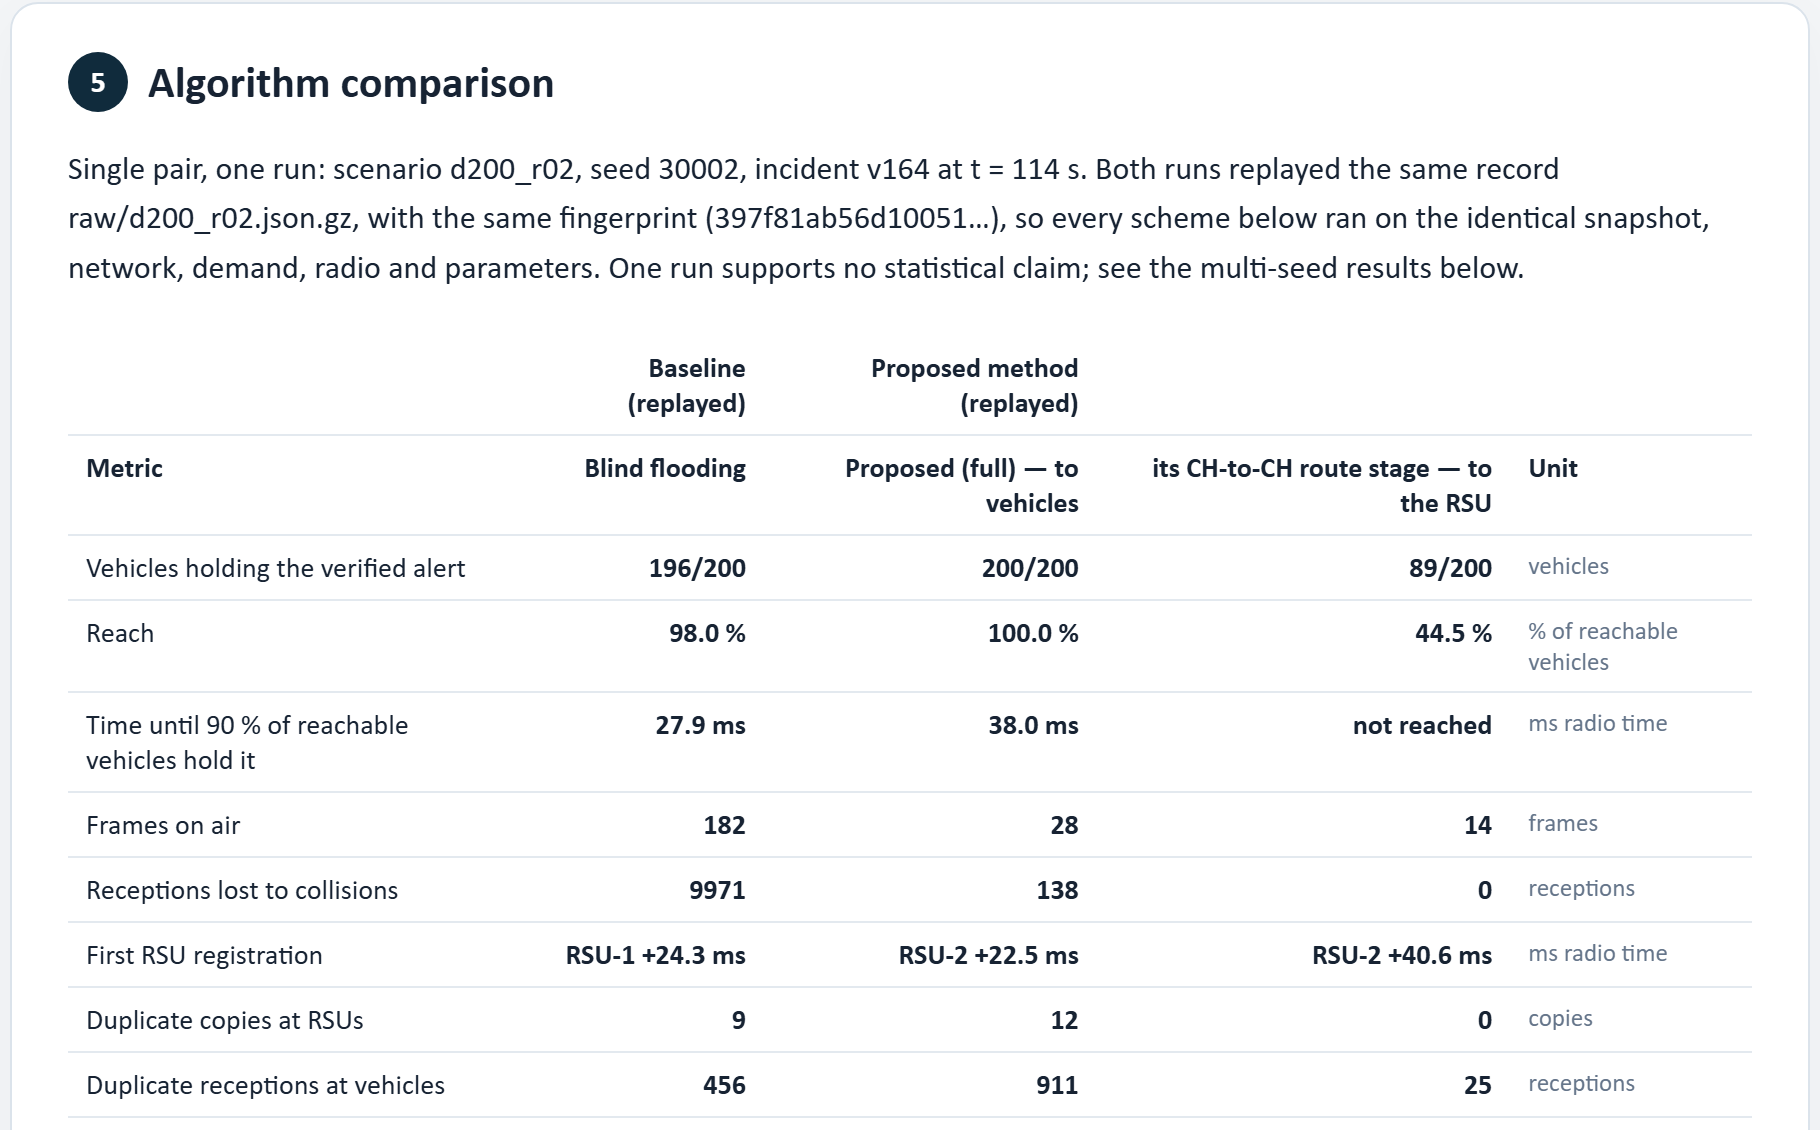
\includegraphics[width=0.9\textwidth]{view_dash_comparison.png}
\caption{Dashboard section 5 for pair P002 (one run of one scenario). \emph{Observe:} blind flooding sent 182 frames and
lost 9971 receptions (196/200 vehicles held the alert); the proposed method sent 28 frames and lost 138 (200/200) but
reached 90\,\% of vehicles about 10 ms later ($t_{90}$ 38.0 ms against 27.9 ms); its CH-to-CH route stage used 14
frames and registered the event at RSU-2 at +40.6 ms. A single pair is an illustration; Section~\ref{sec:results}
gives the statistics.}
\label{fig:dash_comparison}
\end{figure}

\begin{figure}[H]
\centering
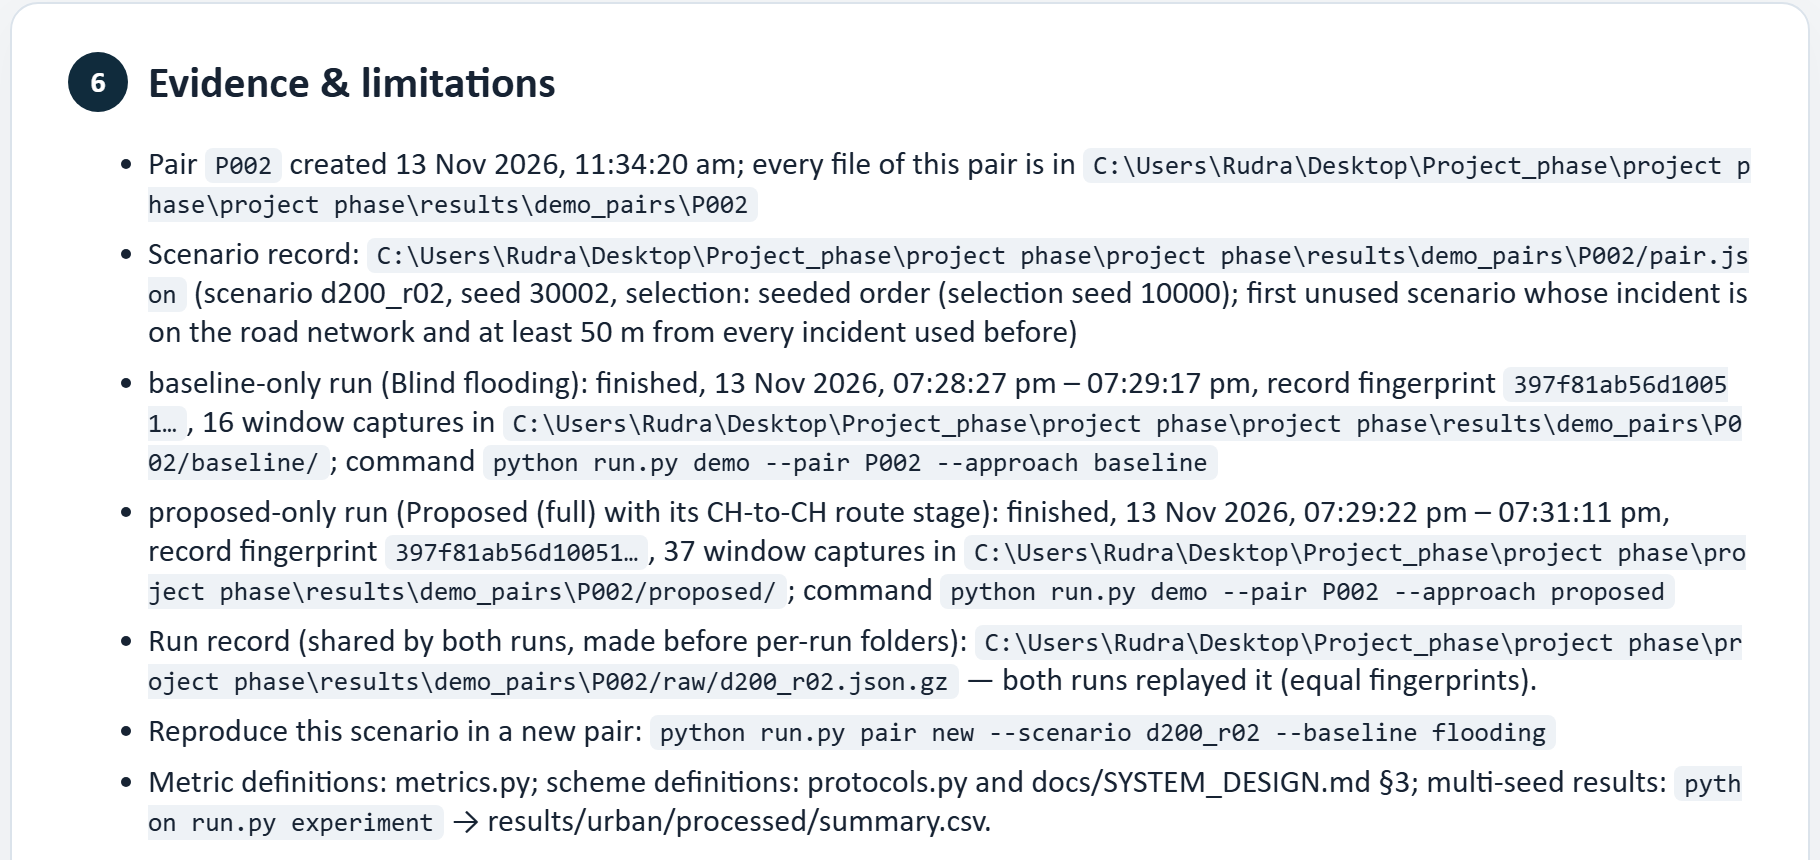
\includegraphics[width=0.9\textwidth]{view_dash_evidence.png}
\caption{Dashboard section 6 (evidence). \emph{Observe:} the folder, record and fingerprint of each run, the number of
window captures, and the commands that reproduce the pair. The same card lists the demonstration's limitations, which
Section~\ref{sec:limits} repeats.}
\label{fig:dash_evidence}
\end{figure}

% =====================================================================
\section{Experimental Setup and Evaluation Metrics}
\label{sec:setup}
\begin{itemize}[noitemsep, topsep=2pt]
  \item \textbf{Experiment matrix.} 6 densities $\times$ 30 seeds = \NScenarios{} scenarios, one alert each. In every
        scenario all schemes run on the \emph{same} snapshot (paired design); each scheme has its own deterministic random
        stream.
  \item \textbf{Schemes.} The four baselines and the proposed method; seven ablations; the CH-to-CH route stage.
  \item \textbf{Forged-alert test.} Same snapshot; a misbehaving vehicle claims an accident that did not happen and up to
        five nearby misbehaving vehicles endorse it. Three protection levels: no voting, voting + BLS without the
        reputation gate, and full protection.
  \item \textbf{Sensitivity sweeps} at 200 vehicles $\times$ 30 seeds: radio range 150, 300 and 450 m; misbehaving
        share 0, 10, 20 and 30\,\%; on-off attackers that relay correctly 0, 50 or 90\,\% of the time while watched.
  \item \textbf{Statistics.} Mean $\pm$ 95\,\% Student-t confidence interval over the runs where a value is defined; $n$ is
        printed when fewer than 30 runs had a value. Comparative claims use \emph{paired} differences per scenario,
        called better or worse only when their 95\,\% CI excludes zero.
  \item \textbf{Verification.} The 105 tests in \texttt{validation/} pass; the experiment command reproduces the stored
        CSVs and figures.
\end{itemize}

\begin{table}[htbp]
\centering
\footnotesize
\renewcommand{\arraystretch}{1.2}
\begin{adjustbox}{max width=\textwidth}
\begin{tabular}{|p{4.4cm}|p{9.2cm}|p{1.6cm}|}
\hline
\textbf{Metric} & \textbf{Definition (\texttt{metrics.py})} & \textbf{Better} \\
\hline
Frames on air & Every frame sent for one alert: proposal, votes and every certified alert & Lower \\
Receptions lost & In-range receptions destroyed by an overlapping transmission & Lower \\
Reach & Vehicles holding the alert / vehicles connected to the source by radio & Higher \\
$t_{90}$ & Time until 90\,\% of reachable vehicles hold the alert (undefined if never reached) & Lower \\
Suppression & SUPPRESS / (SUPPRESS + FORWARD) over honest relaying vehicles & Higher \\
RSU registration & Time until an RSU registered the event (first valid copy + 4.3 ms verification) & Lower \\
Forged alert registered & Runs in which an RSU registered a forged event & Lower \\
\hline
\end{tabular}
\end{adjustbox}
\caption{Evaluation metrics.}
\end{table}

% =====================================================================
\section{Results, Comparison and Discussion}
\label{sec:results}
All five approaches ran on the same \NScenarios{} scenarios. Values are means with a 95\,\% Student-t confidence
interval (CI) over the 30 scenarios of a density; $n$ is printed when fewer runs define a value (for example, $t_{90}$ is
undefined when a run never reaches 90\,\%). Because every scheme runs on the same snapshot, each comparison is also made
as a \emph{paired} difference, proposed minus baseline, per scenario. A difference is called \emph{better} or
\emph{worse} only when its 95\,\% CI excludes zero; otherwise it is called \emph{similar}.

\subsection{Main comparison at 200 vehicles}
Table~\ref{tab:headline} gives the default density. The proposed method has the fewest receptions lost and full reach;
slotted 1-p with random delay has the fewest frames, the highest suppression and the earliest RSU registration;
flooding with random delay has the lowest $t_{90}$.

\begin{table}[H]
\centering
\gentable{tab_headline_200.tex}
\caption{Results at 200 vehicles (30 scenarios, mean $\pm$ 95\,\% CI). Bold marks the best mean of each column, not a
statistically clear win; Table~\ref{tab:verdict} gives the paired verdicts. Source:
\texttt{results/urban/processed/summary.csv}.}
\label{tab:headline}
\end{table}

\subsection{Comparison across densities}
Figures~\ref{fig:chart_frames} and~\ref{fig:chart_reach} repeat the comparison for 50 to 500 vehicles, and
Tables~\ref{tab:frames} and~\ref{tab:t90} give the exact values.

\begin{figure}[H]
\centering
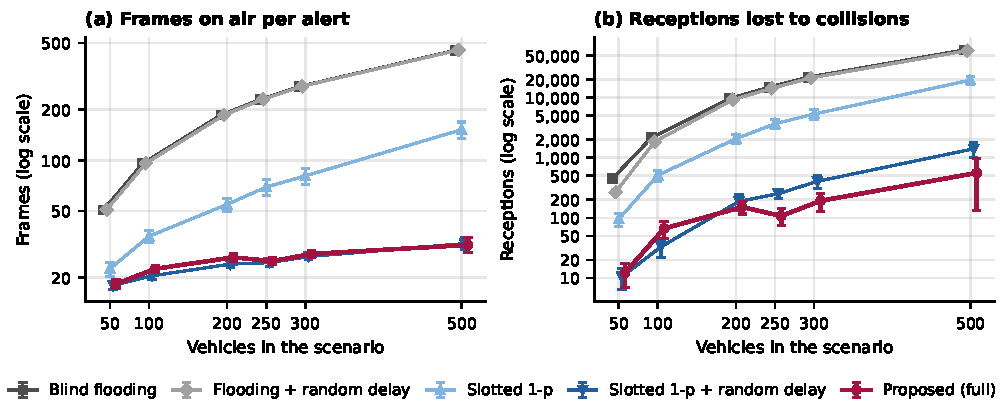
\includegraphics[width=\textwidth]{rep_frames_losses.pdf}
\caption{Frames on air (a) and receptions lost to collisions (b) per alert, by traffic density (log scale; mean
$\pm$ 95\,\% CI, 30 scenarios per point). Flooding grows with density; the proposed method and slotted 1-p with
random delay stay between about 18 and 32 frames.}
\label{fig:chart_frames}
\end{figure}

\begin{figure}[H]
\centering
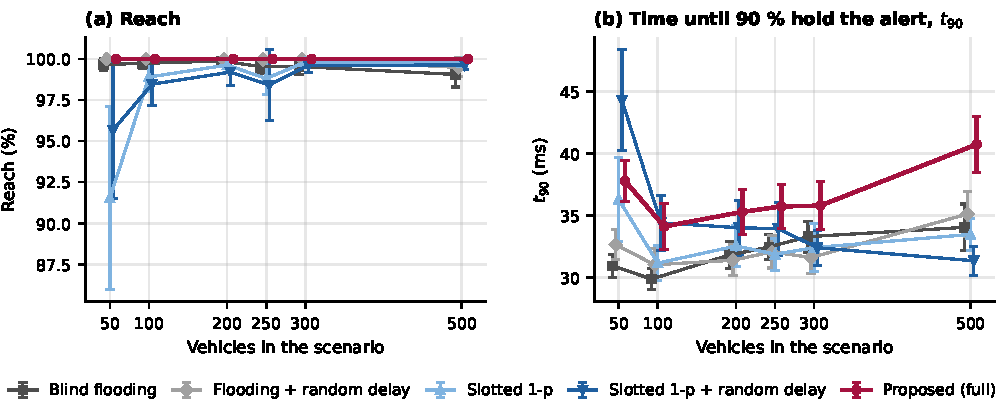
\includegraphics[width=\textwidth]{rep_reach_t90.pdf}
\caption{Reach (a) and the time until 90\,\% of reachable vehicles hold the alert (b), by density (mean $\pm$ 95\,\%
CI). The slotted schemes lose reach at 50 vehicles; the proposed method keeps full reach but is the slowest at 200 to
500 vehicles. Points with fewer than 30 defined runs are listed in Table~\ref{tab:t90}.}
\label{fig:chart_reach}
\end{figure}

\begin{table}[H]
\centering
\gentable{tab_density_frames.tex}
\caption{Frames on air per alert at every density (mean $\pm$ 95\,\% CI).}
\label{tab:frames}
\end{table}

\begin{table}[H]
\centering
\gentable{tab_density_t90.tex}
\caption{$t_{90}$ in ms at every density (mean $\pm$ 95\,\% CI; $n$ shown where fewer than 30 runs reached 90\,\%).}
\label{tab:t90}
\end{table}

\subsection{Better, similar or worse: paired verdicts}
Table~\ref{tab:verdict} compares the proposed method with each baseline at 200 vehicles. Table~\ref{tab:strongest} and
Figure~\ref{fig:chart_strongest} compare it with the strongest baseline, slotted 1-p with random delay, at every density.

\begin{table}[H]
\centering
\gentable{tab_verdict_200.tex}
\caption{Proposed minus each baseline at 200 vehicles (paired, mean $\pm$ 95\,\% CI over 30 scenarios). ``Better'' or
``worse'' only when the CI excludes zero; lower is better for frames, losses, $t_{90}$ and RSU registration, higher for
reach (pp = percentage points).}
\label{tab:verdict}
\end{table}

\begin{table}[H]
\centering
\gentable{tab_verdict_strongest.tex}
\caption{Proposed minus the strongest baseline (slotted 1-p + random delay) at every density, with the same verdict
rule.}
\label{tab:strongest}
\end{table}

\begin{figure}[H]
\centering
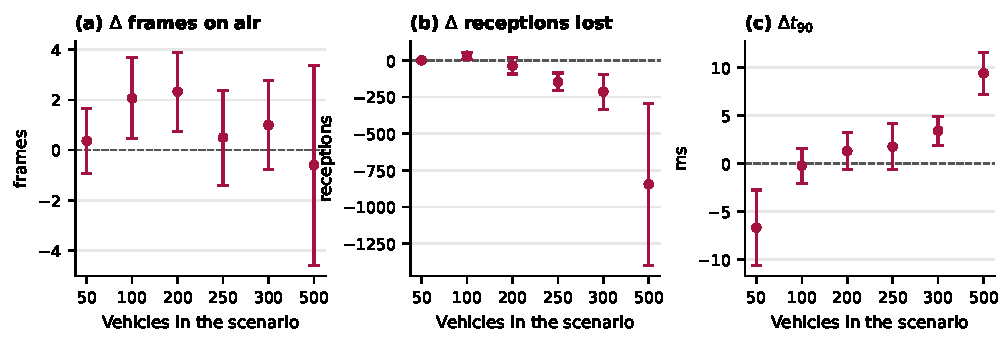
\includegraphics[width=\textwidth]{rep_strongest.pdf}
\caption{Paired differences, proposed minus slotted 1-p + random delay, by density (mean $\pm$ 95\,\% CI; the dashed
line is no difference, below it the proposed method is better). Frames are similar except at 100 and 200 vehicles,
where the proposed method sends about two more; losses are lower from 250 vehicles; $t_{90}$ is lower at 50 vehicles
and higher from 300 vehicles.}
\label{fig:chart_strongest}
\end{figure}

\subsection{What each component contributes (ablation)}
Each ablation removes one component of the proposed method on the same scenarios (Table~\ref{tab:ablation},
Figure~\ref{fig:chart_ablation}).

\begin{table}[H]
\centering
\gentable{tab_ablation_200.tex}
\caption{The proposed method with one component removed, 200 vehicles (mean $\pm$ 95\,\% CI).}
\label{tab:ablation}
\end{table}

\begin{figure}[H]
\centering
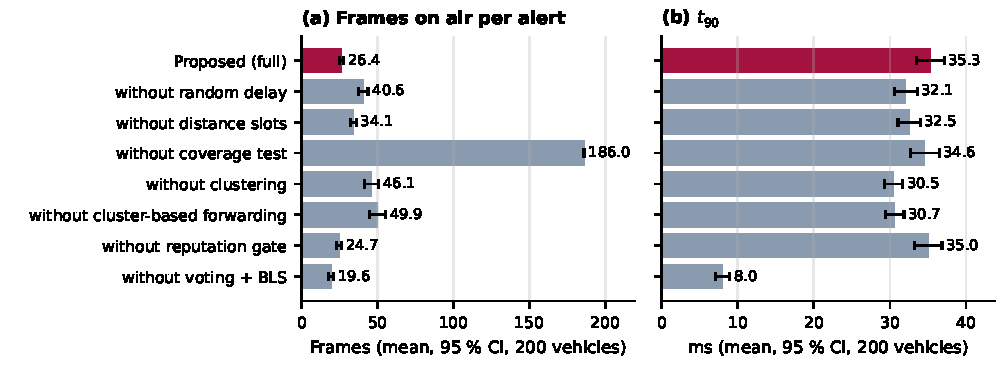
\includegraphics[width=\textwidth]{rep_ablation.pdf}
\caption{Frames on air (a) and $t_{90}$ (b) at 200 vehicles for the full method and each ablation. The coverage test
gives most of the saving; voting and BLS give most of the delay.}
\label{fig:chart_ablation}
\end{figure}

\subsection{Security: forged alerts}
The forged-alert test uses the same traffic with three protection levels; the on-off sweep repeats it against
attackers that behave well part of the time (Table~\ref{tab:forgery}, Figure~\ref{fig:chart_forgery}).

\begin{table}[H]
\centering
\gentable{tab_forgery_200.tex}
\caption{Forged-alert test at 200 vehicles (30 scenarios per row). ``Honest vehicles accepting'' is the mean share of
reachable honest vehicles that accepted the forged alert. Source: \texttt{forgery\_runs.csv} and the on-off sensitivity
sweep.}
\label{tab:forgery}
\end{table}

\begin{figure}[H]
\centering
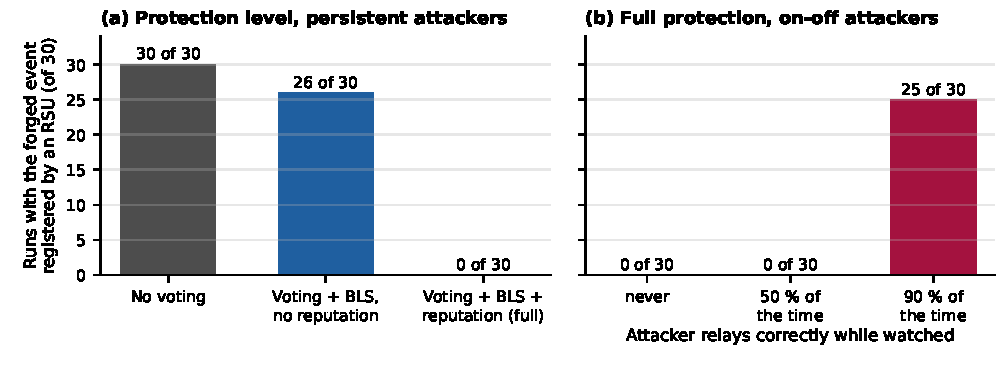
\includegraphics[width=\textwidth]{rep_forgery.pdf}
\caption{Runs in which an RSU registered a forged event, 200 vehicles. (a) By protection level, against persistent
attackers. (b) Full protection against on-off attackers that relay correctly some of the time while watched.}
\label{fig:chart_forgery}
\end{figure}

\subsection{CH-to-CH route stage and radio range}
The route stage is not one of the five broadcast schemes: it runs after the proposed broadcast on the same snapshot
and only aims at the RSU, so its frames are reported separately (Table~\ref{tab:chroute}). Table~\ref{tab:range} shows
the effect of the radio range.

\begin{table}[H]
\centering
\gentable{tab_chroute.tex}
\caption{CH-to-CH route stage: frames on the route, runs in which it registered the event at an RSU, and its registration
time compared with the proposed broadcast (mean $\pm$ 95\,\% CI over runs with a registration).}
\label{tab:chroute}
\end{table}

\begin{table}[H]
\centering
\gentable{tab_range.tex}
\caption{Radio-range sensitivity at 200 vehicles (30 scenarios per range).}
\label{tab:range}
\end{table}

\subsection{Discussion}
\noindent\textbf{Where the proposed method is better.} Against blind flooding, flooding with random delay and slotted
1-persistence it sends far fewer frames and loses far fewer receptions, with the same reach. At 200 vehicles it sent
\NFrProp{} frames against \NFrFlood{} for flooding (about \NCutVsFlood\,\% fewer) and \NFrSlot{} for slotted
1-persistence (about \NCutVsSlot\,\% fewer, paired \NDFrSlot{}~$\pm$~\NDFrSlotCI), and lost \NLossProp{} receptions
against \NLossFlood. The gap widens with density: flooding grows from \NFrFloodFifty{} frames at 50 vehicles to
\NFrFloodFiveH{} at 500, while the proposed method stays between \NFrPropFifty{} and \NFrPropFiveH.

\noindent\textbf{Where it is similar.} Reach at 200 vehicles is statistically the same as every baseline
(Table~\ref{tab:verdict}). Against the strongest baseline, receptions lost at 200 vehicles
(\NDLossSlotRad{}~$\pm$~\NDLossSlotRadCI) and $t_{90}$ at 100 to 250 vehicles (\NDTnSlotRad{}~$\pm$~\NDTnSlotRadCI{} ms at 200) are similar.

\noindent\textbf{Where it is worse.} It is not the fastest. At 200 vehicles its $t_{90}$ is \NTnProp{} ms against
\NTnFlood{} ms for flooding: \NDTnFlood{}~$\pm$~\NDTnFloodCI{} ms paired, and \NDTnFloodRad{} and \NDTnSlot{} ms
against flooding with random delay and slotted 1-persistence. Against the strongest baseline it sends slightly more
frames at 100 and 200 vehicles (\NDFrSlotRadHundred{} and \NDFrSlotRad{} frames), loses more receptions at 100 vehicles
(\NDLossSlotRadHundred{}~$\pm$~\NDLossSlotRadHundredCI), registers at the RSU \NDRsuSlotRad{}~$\pm$~\NDRsuSlotRadCI{} ms
later at 200 vehicles, and is slower in dense traffic (\NDTnSlotRadThreeH{} ms at 300 and
\NDTnSlotRadFiveH{}~$\pm$~\NDTnSlotRadFiveHCI{} ms at 500 vehicles).

\noindent\textbf{The delay cost.} Most of the delay is the price of security, which every approach pays because the
corroboration is shared: three votes release the alert at \NQuorumMs{} ms, and without voting and BLS the proposed
method needs \NFrNoSec{} frames and \NTnNoSec{} ms instead of \NFrProp{} frames and \NTnProp{} ms (\NSecTn{} ms
more). The forwarding rule adds a few milliseconds on top: a vehicle decides only when its timer fires, and tier-1
vehicles wait up to 25 ms behind tier-0 vehicles.

\noindent\textbf{What the strongest baseline achieves.} Slotted 1-p with random delay sent \NFrSlotRad{} frames at 200
vehicles, suppressed \NSupSlotRad\,\% of the relays (proposed \NSupProp\,\%) and registered at the RSU in \NRsuSlotRad{}
ms (proposed \NRsuProp{} ms). It falls behind in sparse traffic: at 50 vehicles it averaged \NReachSlotRadFifty\,\%
reach (paired \NDReachSlotRadFifty{}~$\pm$~\NDReachSlotRadFiftyCI{} pp for the proposed method) and needed
\NTnSlotRadFifty{} ms for $t_{90}$ against \NTnPropFifty{} ms (\NDTnSlotRadFifty{}~$\pm$~\NDTnSlotRadFiftyCI{} ms over the
\NNTnSlotRadFifty{} runs where both reached 90\,\%). In dense traffic the proposed method loses fewer receptions
(\NLossPropFiveH{} against \NLossSlotRadFiveH{} at 500 vehicles, paired
\NDLossSlotRadFiveH{}~$\pm$~\NDLossSlotRadFiveHCI). The proposed method therefore does not beat the strongest baseline overall: frame counts are
similar, it trades a few milliseconds of delay in dense traffic for fewer collisions there and for reach in sparse
traffic, and the full-reach result relies on a radio model without fading.

\noindent\textbf{What the ablations show.} The coverage test gives most of the saving: without it the method sends
\NFrNoCov{} frames, as many as flooding. Clustering and cluster-based forwarding come next (\NFrNoClu{} and \NFrNoCluFwd{}
frames without them; without clustering, \NFrNoCluFiveH{} instead of \NFrPropFiveH{} at 500 vehicles); the random delay
and the distance slots reduce both frames and collisions (\NFrNoRad{} and \NFrNoSlots{} frames without them). Removing the reputation
gate saves about two frames (\NFrNoRep{}), because every vehicle may then become a cluster head or vote, but it is the
gate that stops forged alerts (below).

\noindent\textbf{Security.} Without voting, the forged event was registered in \NForgNoVote{} of 30 runs; with voting
and BLS but no reputation gate in \NForgVoteOnly{} of 30, because three colluders can produce a valid aggregate
signature. With full protection it was registered in \NForgFull{} of 30 runs, but only because default attackers never
relay, so their trust stays at or below 0.5. Attackers that relay correctly 90\,\% of the time earn trust near 0.9 and
got the forged event registered in \NForgOnOffNine{} of 30 runs. The protection therefore works against persistent
misbehaviour, not against on-off attackers.

\noindent\textbf{Sparse networks and the quorum.} Corroboration is fail-closed: if fewer than three trusted neighbours
can vote, the alert is never released. In the main experiment (300 m range) every genuine alert reached its quorum, but
the project audit measured 14 of 30 genuine alerts not released at 50 vehicles with a 150 m range
(\texttt{docs/AUDIT.md}, SCE-1). With a 150 m range at 200 vehicles the network is sparse: the proposed method kept
95.8\,\% reach but needed 127.6 ms for $t_{90}$ and more frames than the strongest baseline (52.5 against 32.2), which
in turn reached only 65.4\,\% (Table~\ref{tab:range}). At 450 m it sent the fewest frames of all (18.1 against 20.3).

\noindent\textbf{CH-to-CH route stage.} The route used about \NFrRoute{} frames at 200 vehicles and registered the event
in \NRsuRouteRuns{} of 30 runs, in \NRsuRoute{} ms on average, later than the broadcast's \NRsuProp{} ms. Its frames come
on top of the broadcast (about \NFrPropPlusRoute{} frames per alert when both run). It is a second, corroborated
delivery path to the RSU that writes the event to the local store; it does not replace the broadcast to vehicles and has
no fallback when the route or a local quorum fails.

% =====================================================================
\section{Design Choices and Trade-offs}
\begin{itemize}[noitemsep, topsep=2pt]
  \item \textbf{DBSCAN} needs no preset number of clusters, which suits traffic, and marks isolated vehicles (bridges)
        that often link two groups.
  \item \textbf{Beta reputation} starts at 0.5 and moves slowly, so one wrong observation does not ruin an honest vehicle.
        The 0.7 threshold separates persistent misbehaviour from honest vehicles but, as measured, not on-off attackers.
  \item \textbf{BLS aggregation} keeps the certificate at 96 bytes for any number of signers, so the alert size grows only
        by 4 bytes per signer ID.
  \item \textbf{Coverage test} uses neighbour lists that vehicles already have from beacons, so it needs no extra
        messages. Its cost is per-vehicle set operations over the heard senders' neighbour lists.
  \item \textbf{Complexity.} Neighbour tables and DBSCAN use pairwise distances, $O(n^2)$ for $n$ vehicles: acceptable at
        500 vehicles on a laptop (the whole experiment takes about 162 s).
  \item \textbf{Fail-closed corroboration.} If fewer than three trusted neighbours can vote, the alert is never released.
        We chose this so that an uncorroborated alert can never spread; the price is that a genuine alert can be lost in
        sparse traffic (Section~\ref{sec:results}, \emph{Sparse networks and the quorum}).
  \item \textbf{Shared corroboration.} All five approaches use the same committee, certificate and RSU checks, so the
        comparison isolates the forwarding rule. The baselines here are therefore not the unprotected originals from the
        literature: they check the same certificate, and the security cost (about \NSecTn{} ms of $t_{90}$) appears in
        every column.
\end{itemize}

% =====================================================================
\section{Limitations}
\label{sec:limits}
\begin{itemize}[noitemsep, topsep=2pt]
  \item Everything runs in simulation. The radio is a unit-disk model (fixed 300 m range) without fading, capture or
        background beacon load, so real performance will be worse.
  \item The road network is a small $5\times5$ grid with two RSUs; no highway or real city map was tested.
  \item Trust detection is easy in the default setting (persistent black holes). On-off attackers pass the trust gate
        (\NForgOnOffNine{} of 30 forged events registered).
  \item Keys are derived from vehicle IDs: there is no certificate authority, revocation or privacy protection.
  \item Fail-closed corroboration can drop genuine alerts in sparse traffic; the specified quorum-timeout fallback is not
        implemented.
  \item The CH-to-CH route has no fallback when the route or a local quorum fails.
  \item The RSU does not rebroadcast; the traffic centre is a local outbox and the cloud store is a local SQLite database
        unless an endpoint is configured. Several reports of one crash are merged only by a conservative rule that the
        simulation (one report per incident) exercises in unit tests only.
  \item The SUMO-GUI demonstration replays a recorded run on the identical SUMO state; the radio is not computed inside
        the GUI process.
\end{itemize}

% =====================================================================
\section{Conclusion and Future Scope}
\noindent\textbf{Conclusion.} We implemented the full path from SUMO traffic to a registered, corroborated emergency
alert and evaluated it on \NScenarios{} paired scenarios against four implemented baselines. Trust-aware clustering with a
coverage test cut the frames per alert by about \NCutVsFlood\,\% against blind flooding and about \NCutVsSlot\,\% against
slotted 1-persistence at 200 vehicles, for a few milliseconds of extra delay. It does not beat the strongest baseline,
slotted 1-persistence with random delay, overall: frame counts are similar (about two more at 100 and 200 vehicles),
collisions are fewer in dense traffic and reach is higher in sparse traffic, while $t_{90}$ is higher in dense traffic.
Corroboration with BLS certificates stopped forged alerts from persistently misbehaving vehicles, but not from
attackers who first build a good record (\NForgOnOffNine{} of 30 forged events registered), and it can withhold a
genuine alert when too few trusted neighbours are in range. The demonstration and dashboard show each result on real
SUMO-GUI runs and tie every displayed number to its recorded run.

\noindent\textbf{Future scope.}
\begin{itemize}[noitemsep, topsep=2pt]
  \item A fading radio model with beacon load, and validation with a network simulator or real 802.11p hardware.
  \item Larger and real road networks (e.g.\ OpenStreetMap maps) and more RSUs.
  \item A reputation that resists on-off attackers, a real public-key infrastructure, and the quorum-timeout fallback.
  \item A fallback for the CH-to-CH route and tuning of the slot, delay and committee parameters.
  \item Sensor-based crash detection with several reporters per incident.
\end{itemize}

% =====================================================================
\section{Project Deliverables \& Technical Enrichment Summary}
\begin{table}[H]
    \centering
    \footnotesize
    \renewcommand{\arraystretch}{1.2}
    \begin{tabular}{|>{\raggedright\arraybackslash}p{3.3cm}|>{\raggedright\arraybackslash}p{9.8cm}|>{\raggedright\arraybackslash}p{2.3cm}|}
        \hline
        \textbf{Deliverable Category} & \textbf{Details / Title / Repository Link} & \textbf{Status} \\
        \hline
        Source Code Repository & Public GitHub repository \url{https://github.com/AkhilRudrapaka/IoV-Emergency-Broadcast}: source
        code, README, documentation, validation tests and stored results. Last pushed 27 Oct 2026; the later local work
        described in this report is not yet in the public copy & Completed \\
        \hline
        Project Implementation Report and Presentation & This report and the panel presentation
        (\texttt{final\_panel\_review/}) & Completed \\
        \hline
        Individual Online Certifications & Every member completed \emph{Introduction to the Internet of Things and Embedded
        Systems} (University of California, Irvine, on Coursera): \StudentA{} (\RegA), \StudentB{} (\RegB), \StudentC{}
        (\RegC), \StudentD{} (\RegD), \StudentE{} (\RegE). Certificates dated 20--22 Oct 2026; all five confirmed on
        Coursera's verification pages & Completed\newline (5 of 5) \\
        \hline
        Group TEA Deliverable 1 -- Online Course & Team course \emph{Introduction to the Internet of Things and Embedded
        Systems}, University of California, Irvine (Coursera): five completion certificates and a course relevance report
        that relates the course to this project & Completed \\
        \hline
        Group TEA Deliverable 2 -- Research Paper & Manuscript \emph{Trust-Aware Cluster-Based Broadcast Suppression for
        Real-Time Vehicular Emergency Alerts} (8 pages, prepared 17 Oct 2026); not yet published or accepted & Completed
        (manuscript) \\
        \hline
        Group TEA Deliverable 3 -- Project Documentation Website & \url{https://iov-documentation-portal.vercel.app/}:
        project documentation portal, reachable on 15 Nov 2026 (the deployed version is the portal of 27 Oct 2026) &
        Completed \\
        \hline
    \end{tabular}
    \caption{Summary of Completed Project and Technical Enrichment Deliverables}
\end{table}

% --- REFERENCES ---
\vspace{0.2cm}
\nocite{*}
\renewcommand{\refname}{\large\bfseries\color{amritaMaroon}References}
\bibliographystyle{ieeetr}
\begingroup\small
\bibliography{references}
\endgroup

\end{document}
